% !TeX spellcheck = hu_HU
% !TeX encoding = UTF-8
% !TeX program = xelatex
% TODO Change language to en_GB (recommended) or en_US for English documents
\documentclass[11pt,a4paper,oneside]{report}             % Single-side
%\documentclass[11pt,a4paper,twoside,openright]{report}  % Duplex

% thanks to http://tex.stackexchange.com/a/47579/71109
\usepackage{ifxetex}
\usepackage{ifluatex}
\newif\ifxetexorluatex % a new conditional starts as false
\ifnum 0\ifxetex 1\fi\ifluatex 1\fi>0
   \xetexorluatextrue
\fi

\ifxetexorluatex
  \usepackage{fontspec}
\else
  \usepackage[T1]{fontenc}
  \usepackage[utf8]{inputenc}
  \usepackage[lighttt]{lmodern}
\fi

\usepackage[english,magyar]{babel} % Alapértelmezés szerint utoljára definiált nyelv lesz aktív, de később külön beállítjuk az aktív nyelvet.

%\usepackage{cmap}
\usepackage{amsfonts,amsmath,amssymb} % Mathematical symbols.
%\usepackage[ruled,boxed,resetcount,linesnumbered]{algorithm2e} % For pseudocodes. % beware: this is not compatible with LuaLaTeX, see http://tex.stackexchange.com/questions/34814/lualatex-and-algorithm2e
\usepackage{booktabs} % For publication quality tables for LaTeX
\usepackage{graphicx}

%\usepackage{fancyhdr}
%\usepackage{lastpage}

\usepackage{anysize}
%\usepackage{sectsty}
\usepackage{setspace} % For setting line spacing

\usepackage[unicode]{hyperref} % For hyperlinks in the generated document.
\usepackage{xcolor}
\usepackage{listings} % For source code snippets.

\usepackage[amsmath,thmmarks]{ntheorem} % Theorem-like environments.

\usepackage[hang]{caption}

\singlespacing

\newcommand{\selecthungarian}{
	\selectlanguage{magyar}
	\setlength{\parindent}{2em}
	\setlength{\parskip}{0em}
	\frenchspacing
}

\newcommand{\selectenglish}{
	\selectlanguage{english}
	\setlength{\parindent}{0em}
	\setlength{\parskip}{0.5em}
	\nonfrenchspacing
	\renewcommand{\figureautorefname}{Figure}
	\renewcommand{\tableautorefname}{Table}
	\renewcommand{\partautorefname}{Part}
	\renewcommand{\chapterautorefname}{Chapter}
	\renewcommand{\sectionautorefname}{Section}
	\renewcommand{\subsectionautorefname}{Section}
	\renewcommand{\subsubsectionautorefname}{Section}
}

\usepackage[numbers]{natbib}
\usepackage{xspace}
\usepackage{float}


%TODO Set the main variables
\newcommand{\vikszerzoVezeteknev}{Arany}
\newcommand{\vikszerzoKeresztnev}{Dániel}

\newcommand{\vikkonzulensAMegszolitas}{dr.~}
\newcommand{\vikkonzulensAVezeteknev}{Kovácsházy}
\newcommand{\vikkonzulensAKeresztnev}{Tamás}

\newcommand{\vikkonzulensBMegszolitas}{}
\newcommand{\vikkonzulensBVezeteknev}{}
\newcommand{\vikkonzulensBKeresztnev}{}

\newcommand{\vikkonzulensCMegszolitas}{}
\newcommand{\vikkonzulensCVezeteknev}{}
\newcommand{\vikkonzulensCKeresztnev}{}

\newcommand{\vikcim}{Using Rust on Multicore Microcontrollers} % Cím
\newcommand{\viktanszek}{\bmemit} % Tanszék
\newcommand{\vikdoktipus}{\msc} % Dokumentum típusa (\bsc vagy \msc)
\newcommand{\vikmunkatipusat}{diplomaterv} % a "hallgató nyilatkozat" részhez: szakdolgozatot vagy diplomatervet

\input{include/tdk-variables}
\newcommand{\szerzoMeta}{\vikszerzoVezeteknev{} \vikszerzoKeresztnev} % egy szerző esetén
%\newcommand{\szerzoMeta}{\vikszerzoVezeteknev{} \vikszerzoKeresztnev, \tdkszerzoB} % két szerző esetén

%TODO Language configuration -- choose one
% Beállítások magyar nyelvű dolgozathoz
%\input{include/thesis-hu}
% Settings for English documents
\input{include/thesis-en}

%--------------------------------------------------------------------------------------
% Page layout setup
%--------------------------------------------------------------------------------------
% we need to redefine the pagestyle plain
% another possibility is to use the body of this command without \fancypagestyle
% and use \pagestyle{fancy} but in that case the special pages
% (like the ToC, the References, and the Chapter pages)remain in plane style

\pagestyle{plain}
\marginsize{35mm}{25mm}{15mm}{15mm}

\setcounter{tocdepth}{3}
%\sectionfont{\large\upshape\bfseries}
\setcounter{secnumdepth}{3}

\sloppy % Margón túllógó sorok tiltása.
\widowpenalty=10000 \clubpenalty=10000 %A fattyú- és árvasorok elkerülése
\def\hyph{-\penalty0\hskip0pt\relax} % Kötőjeles szavak elválasztásának engedélyezése


%--------------------------------------------------------------------------------------
% Setup hyperref package
%--------------------------------------------------------------------------------------
\hypersetup{
    % bookmarks=true,            % show bookmarks bar?
    unicode=true,              % non-Latin characters in Acrobat's bookmarks
    pdftitle={\vikcim},        % title
    pdfauthor={\szerzoMeta},    % author
    pdfsubject={\vikdoktipus}, % subject of the document
    pdfcreator={\szerzoMeta},   % creator of the document
    pdfproducer={},    % producer of the document
    pdfkeywords={},    % list of keywords (separate then by comma)
    pdfnewwindow=true,         % links in new window
    colorlinks=true,           % false: boxed links; true: colored links
    linkcolor=black,           % color of internal links
    citecolor=black,           % color of links to bibliography
    filecolor=black,           % color of file links
    urlcolor=black             % color of external links
}


%--------------------------------------------------------------------------------------
% Set up listings
%--------------------------------------------------------------------------------------
\definecolor{lightgray}{rgb}{0.95,0.95,0.95}
\lstset{
	basicstyle=\scriptsize\ttfamily, % print whole listing small
	keywordstyle=\color{black}\bfseries, % bold black keywords
	identifierstyle=, % nothing happens
	% default behavior: comments in italic, to change use
	% commentstyle=\color{green}, % for e.g. green comments
	stringstyle=\scriptsize,
	showstringspaces=false, % no special string spaces
	aboveskip=3pt,
	belowskip=3pt,
	backgroundcolor=\color{lightgray},
	columns=flexible,
	keepspaces=true,
	escapeinside={(*@}{@*)},
	captionpos=b,
	breaklines=true,
	frame=single,
	float=!ht,
	tabsize=2,
	literate=*
		{á}{{\'a}}1	{é}{{\'e}}1	{í}{{\'i}}1	{ó}{{\'o}}1	{ö}{{\"o}}1	{ő}{{\H{o}}}1	{ú}{{\'u}}1	{ü}{{\"u}}1	{ű}{{\H{u}}}1
		{Á}{{\'A}}1	{É}{{\'E}}1	{Í}{{\'I}}1	{Ó}{{\'O}}1	{Ö}{{\"O}}1	{Ő}{{\H{O}}}1	{Ú}{{\'U}}1	{Ü}{{\"U}}1	{Ű}{{\H{U}}}1
}


%--------------------------------------------------------------------------------------
% Set up theorem-like environments
%--------------------------------------------------------------------------------------
% Using ntheorem package -- see http://www.math.washington.edu/tex-archive/macros/latex/contrib/ntheorem/ntheorem.pdf

\theoremstyle{plain}
\theoremseparator{.}
\newtheorem{example}{\pelda}

\theoremseparator{.}
%\theoremprework{\bigskip\hrule\medskip}
%\theorempostwork{\hrule\bigskip}
\theorembodyfont{\upshape}
\theoremsymbol{{\large \ensuremath{\centerdot}}}
\newtheorem{definition}{\definicio}

\theoremseparator{.}
%\theoremprework{\bigskip\hrule\medskip}
%\theorempostwork{\hrule\bigskip}
\newtheorem{theorem}{\tetel}


%--------------------------------------------------------------------------------------
% Some new commands and declarations
%--------------------------------------------------------------------------------------
\newcommand{\code}[1]{{\upshape\ttfamily\scriptsize\indent #1}}
%\newcommand{\mycode}{\texttt}
\newcommand{\mycode}[1]{\colorbox{lightgray}{\lstinline[language=C]$#1$}}
\newcommand{\doi}[1]{DOI: \href{http://dx.doi.org/\detokenize{#1}}{\raggedright{\texttt{\detokenize{#1}}}}} % A hivatkozások közt így könnyebb DOI-t megadni.

\DeclareMathOperator*{\argmax}{arg\,max}
%\DeclareMathOperator*[1]{\floor}{arg\,max}
\DeclareMathOperator{\sign}{sgn}
\DeclareMathOperator{\rot}{rot}


%--------------------------------------------------------------------------------------
% Setup captions
%--------------------------------------------------------------------------------------
\captionsetup[figure]{
	width=.75\textwidth,
	aboveskip=10pt}

\renewcommand{\captionlabelfont}{\bf}
%\renewcommand{\captionfont}{\footnotesize\it}

%--------------------------------------------------------------------------------------
% Hyphenation exceptions
%--------------------------------------------------------------------------------------
\hyphenation{Shakes-peare Mar-seilles ár-víz-tű-rő tü-kör-fú-ró-gép}


\author{\vikszerzo}
\title{\viktitle}

% Define the Rust language for listings
\lstdefinelanguage{Rust}{
  sensitive=true,
  keywords=[1]{as, break, const, continue, crate, else, enum, extern, false, fn, for, if, impl, in, let, loop, match, mod, move, mut, pub, ref, return, self, Self, static, struct, super, trait, true, type, unsafe, use, where, while},
  keywords=[2]{bool, char, f32, f64, i8, i16, i32, i64, isize, u8, u16, u32, u64, usize, str},
  keywords=[3]{Some, None, Ok, Err, Result, Option},
  morecomment=[l]{//},
  morecomment=[s]{/*}{*/},
  morestring=[b]{"},
  morestring=[b]{'},
}

% Define your custom style for Rust code
\lstdefinestyle{customrust}{
  belowcaptionskip=1\baselineskip,
  breaklines=true,
  xleftmargin=\parindent,
  language=Rust,
  showstringspaces=false,
  basicstyle=\footnotesize\ttfamily,
  keywordstyle=[1]\color{blue},
  keywordstyle=[2]\color{purple},
  keywordstyle=[3]\color{orange},
  commentstyle=\itshape\color{green!40!black},
  stringstyle=\color{brown},
}

%--------------------------------------------------------------------------------------
% Table of contents and the main text
%--------------------------------------------------------------------------------------
\begin{document}

\pagenumbering{gobble}

%TODO These includes define guidelines -- remove these
%~~~~~~~~~~~~~~~~~~~~~~~~~~~~~~~~~~~~~~~~~~~~~~~~~~~~~~~~~~~~~~~~~~~~~~~~~~~~~~~~~~~~~~
%\include{include/guideline}
%\include{include/project}

\selectthesislanguage

%TODO Titlepage -- choose one from below
%~~~~~~~~~~~~~~~~~~~~~~~~~~~~~~~~~~~~~~~~~~~~~~~~~~~~~~~~~~~~~~~~~~~~~~~~~~~~~~~~~~~~~~
\include{include/titlepage}		   % Szakdolgozat/Diplomaterv címlap
%\include{include/titlepage-tdk}	% TDK címlap
%\include{include/titlepage-otdk}   % OTDK címlap


% Table of Contents
%~~~~~~~~~~~~~~~~~~~~~~~~~~~~~~~~~~~~~~~~~~~~~~~~~~~~~~~~~~~~~~~~~~~~~~~~~~~~~~~~~~~~~~
\tableofcontents\vfill


% Declaration and Abstract
%~~~~~~~~~~~~~~~~~~~~~~~~~~~~~~~~~~~~~~~~~~~~~~~~~~~~~~~~~~~~~~~~~~~~~~~~~~~~~~~~~~~~~~
%\include{include/declaration} %TODO Hallgatói nyilatkozat -- TDK és OTDK esetén törlendő!
\pagenumbering{roman}
\setcounter{page}{1}

\selecthungarian

%----------------------------------------------------------------------------
% Abstract in Hungarian
%----------------------------------------------------------------------------
\chapter*{Kivonat}\addcontentsline{toc}{chapter}{Kivonat}

A jelenleg a legelterjedtebb rendszer programozási nyelvek (C/C++) bizonyos megfontolások mentén elavultnak tekinthetők, mind biztonságos memóriakezelés, mind modern nyelvi elemek tekintetében. A Rust programozási nyelv megoldást kínál ezen nyelvek sok gyakori problémájára, úgy mint a memóriaszivárgások vagy a nem egységes hibakezelés. A fejlesztők körében is egyre elfogadottabb a nyelv, például még a Linux Kernelben is támogatást kapott, a C nyelv után elsőként.\cite{FirstRustCommit}

Ezen kívül egyre több olyan beágyazott rendszer készül, melynek igényeit a legjobban egy többmagos mikrokontroller tudja kielégíteni. A legtöbb nagy gyártó egymagos, mikrokontrollereire már lehet Rust kódból binárist fordítani, azonban többmagos kontrollerek esetében már nem ilyen széles körű a támogatás. Így adott a feladat, hogy a létező többmagos Rust keretrendszereket adaptáljuk az általunk választott többmagos mikrokontrollerhez.

A dolgozat célja, hogy feltérképezze a mikrokontrollerek Rust támogatását, és azt, hogy ez a támogatás hogyan adaptálható többmagos esetekre. Megvizsgálom a többmagos működésére jellemző elemek, mint például szemaforok és üzenetsorok használatát Rust programozási nyelven. Megismerkedek a már rendelkezésre álló megoldásokkal, és adaptálok egyet a kiválasztott többmagos mikrokontrollerre. Végül összehasonlítást végzek egy megszokott C nyelvű többmagos és egy többmagos Rust projekt között.

Egy projekt váz elkészítése után pedig egy többmagos példaalkalmazás készítésével fogom demonstrálni a többmagos Rust lehetőségeit. A fejlesztés során az STM32H745 chip-pel felszerelt Nucleo-H745 fejlesztői kártyát fogom használni, melyen egy Arm Cortex-M7 és egy Cortex-M4 mag található.

A példaalkalmazás keretében a Cortex-M7 mag egy egyszerű webszervert fog megvalósítani és az ethernet periférián keresztül fog csatlakozni egy helyi hálózatra. A Cortex-M4 mag digitális szűrést fog végrehajtani a mikrokontroller egyik analóg bemenetén érkező jelfolyamra és egy analóg kimenetén fogja szolgáltatni ennek eredményét. A szűrés paramétereit a webszerver által hosztolt oldalon lehet majd beállítani. A két mag biztonságos adatcseréjét hardveres szemafor fogja lehetővé tenni.

\vfill
\selectenglish


%----------------------------------------------------------------------------
% Abstract in English
%----------------------------------------------------------------------------
\chapter*{Abstract}\addcontentsline{toc}{chapter}{Abstract}

Currently, the most widely used system programming languages (C/C++) could be considered outdated or old-fashioned, considering both memory safety and modern language features. The Rust programming language aims to solve the most common problems of these older languages, such as memory leaks or non-unified error handling. It is ever more accepted in the developer community, for example, Rust was the first system programming language that got accepted into the Linux kernel besides C. \cite{FirstRustCommit}

More and more embedded systems are made with features that are best satisfied by a multi-core microcontroller system. Many of the big microcontroller manufacturers already support Rust for their single-core controllers but multi-core Rust is not at all widely supported. So the task of adapting the existing multi-core rust environments to a chosen multi-core microcontroller is given.

The purpose of this thesis is to explore the Rust support of microcontrollers, and the adaptation of this support for multi-core ones. I will examine the Rust usage of features prevalent in a multi-core system, such as semaphores and message queues. I will also explore the currently available rust multi-core solutions and adapt one of them to a selected multi-core microcontroller. Finally, I will compare the advantages and disadvantages of the selected framework with a tried and tested C language project structure.

After creating a Rust project skeleton, an example multi-core application will also be developed. During the task, I will use the Nucleo-H745 development board, which has an STM32H45 chip. This chip has an ARM Cortex-M7 and a Cortex-M4 core.

In the example application, the Cortex-M7 core will serve as a simple web server using the ethernet peripheral of the board to connect to a local network. The Cortex-M4 core is going to perform filtering on a signal stream coming through one of the analog pins of the microcontroller, while an analog output will be used to show the result. The parameters of the filtering are going to be configurable from the site hosted by the web server. The safe data flow between the two cores will be guaranteed by a hardware semaphore.


\vfill
\selectthesislanguage

\newcounter{romanPage}
\setcounter{romanPage}{\value{page}}
\stepcounter{romanPage}
    %TODO Összefoglaló -- TDK és OTDK esetén nem kötelező


% The main part of the thesis
%~~~~~~~~~~~~~~~~~~~~~~~~~~~~~~~~~~~~~~~~~~~~~~~~~~~~~~~~~~~~~~~~~~~~~~~~~~~~~~~~~~~~~~
\pagenumbering{arabic}

%TODO import your own content
%----------------------------------------------------------------------------
\chapter{\bevezetes}
%----------------------------------------------------------------------------

The most used language in embedded systems today is without a doubt the C language, followed not so closely by C++. While these languages can get the job done in a microcontroller system, they certainly have some shortcomings, such as lacking real memory safety and features present in more modern languages. Rust aims to solve all these problems so using it in microcontroller driven systems is beneficial.

Rust is supported on an ever growing group of microcontrollers. In this project, besides discussing general aspects of Rust development on a microcontroller, I will use a development board with the STM32H745 dual-core chip. Crucially, most of the STM32 controllers have official Rust support and even some development boards. This support however does not extend to the second core of these microcontrollers as these are, as of writing this thesis, a fairly new product of the manufacturer.

During the first part of the project, I will examine how the 2 cores of this MCU work and work together in a conventional C project, and note any hardware peripherals that are useful in inter-core communication or synchronization. After having an understanding of how an example C project works, I will start to develop a Rust project skeleton, that could be used for larger dual-core applications.

While creating the Rust skeleton project, I will research and document the current status of multi-core Rust development and existing solutions. Then I will discuss the possibilities of setting up a dual-core project for this specific microcontroller, and select one that is most appropriate for my task.

Using the selected method and framework, I will test if the capabilities present in a C project could still be used in the new Rust system. If everything is in order, I will create an example dual-core application based on the Rust project skeleton. This will be the second part of this project.

\chapter{The Rust Programming Language}

This chapter is a brief introduction to the Rust programming language and its most important features in the context of this thesis.

\section{A compiled system programming language}

Officially Rust is considered a system programming language which means that its primary function is performance and ease of access to the hardware while still providing higher-level programming concepts such as data structures to hold and organize data. \cite{SystemProgrammingLanguageWikipedia} For example, in Rust, we can find a dynamic string type, but may also choose to take it as a byte array and manipulate the data that way.

Much like C and C++, Rust programs can only be run after they have been compiled into a binary. The aforementioned higher-level concepts only exist at compile time so the binary program can be as efficient as possible. This will be true for all further concepts explained in this section, the resulting binaries from a C and Rust program are comparable both in size and execution speed, only, the Rust compiler is more sophisticated than the C compiler.

\section{Type system}

\subsection{Types on the stack}

\subsubsection{Simple types}

These are the very basic types of Rust representing numbers, booleans, and characters. Unlike in C, the size of the following types is not implementation-dependent.

For representing numbers one can use \mycode{u8}, \mycode{u16}, \mycode{u32}, \mycode{u64}, \mycode{u128} and \mycode{usize} for representing unsigned integers, where the last one will use as many bits as the platform the code is compiled for (usually 32 or 64). Exchanging the \mycode{u} for an \mycode{i} in these types gives us the signed integer types.

Floating point numbers can be either stored using the \mycode{f32} or the \mycode{f64} type, this is similar to \mycode{float} and \mycode{double} in C.

Characters are represented in memory by 4 bytes to accommodate encodings up to UTF-8.

Rust also has a boolean type which is important for control flow, for example, the \mycode{if} expression only allows a boolean expression in its header.

\subsubsection{Enums and Structs}

It is often said that Rust has an algebraic type system. What this mainly refers to is that all the available types can be combined in two ways. A struct will contain every type from its definition at the same time, while an enum will always evaluate to one of the types listed in its definition.

Enums and Structs also count as complete types which means that unlike in C, they cannot be represented as their underlying types by clever pointer arithmetics.

While structs behave mostly the same way as structs in C or classes in C++, enums are different from these common languages. For example, an enum could be created to represent color encoding types: RGB and hex codes.

\begin{lstlisting}[language=Rust,frame=single,float=!ht,style=customrust,label={lst:rust-enum},caption={Rust Enum Example}]
    enum ColorFormat {
        RGB,
        HexCode
    }
\end{lstlisting}

In Rust, we can go further, and attach relevant data directly to the enum values.

\begin{lstlisting}[language=Rust,frame=single,float=!ht,style=customrust,label={lst:rust-enum-advanced},caption={Rust Enum Example With Data}]
    enum ColorFormat {
        RGB(u8, u8, u8),
        HexCode(String)
    }
\end{lstlisting}

This way when a \mycode{ColorFormat} type is passed to a function, it can determine the incoming color format and also access the color itself. In addition to this, the compiler will check if this function does something with each of the enums it can receive, and fails the compilation if, for example, \mycode{HexCode} type of color format is not handled.

\subsection{Types on the heap}

These are the types where ownership and references are important questions. A good example would be a string, where multiple parts of our code would like to modify or read the value, but ideally, we only want one owner that is responsible for freeing up the memory used when the string is not needed anymore. Most of the types that contain data on the heap are part of the standard library of Rust. These include the aforementioned strings and some containers like \mycode{Vector}. How Rust handles these data types will be discussed further.

\subsection{Type conversions}

There are no implicit conversions between types in Rust. If we have a function in C that expects a \mycode{uint32\_t} as an argument and we try to pass it a variable of \mycode{uint16\_t} type, we may not even get a warning from the compiler and certainly not an error, as implicit type conversion is a part of C and C++. In Rust, however, passing a \mycode{u16} type variable to a function that expects the \mycode{u32} type will result in a compile error. The compiler signals this inconsistency and suggests a solution.

\begin{lstlisting}[language=C,frame=single,float=!ht,label={lst:rust-conv-error},caption={Rust Type Conversion Error}]
    error[E0308]: mismatched types
    --> src/main.rs:7:15
     |
   7 |     print_u32(mynum);
     |     --------- ^^^^^ expected `u32`, found `u16`
     |     |
     |     arguments to this function are incorrect
     |
   note: function defined here
    --> src/main.rs:1:4
     |
   1 | fn print_u32(num: u32) {
     |    ^^^^^^^^^ --------
   help: you can convert a `u16` to a `u32`
     |
   7 |     print_u32(mynum.into());
     |                    +++++++

   For more information about this error, try `rustc --explain E0308`.
\end{lstlisting}

When we try to reverse the types in our example, C issues a warning about truncating integers, but still many programmers can just ignore this warning and assume the data is properly sanitized. Rust obviously will not let a code compile with integer truncation, but the solution is a bit more complex this time because a possibility is present that the value does not fit in the smaller type.

\begin{lstlisting}[language=C,frame=single,float=!ht,label={lst:rust-reverse-conv-error},caption={Rust Type Conversion Error}]
    error[E0308]: mismatched types
    --> src/main.rs:7:15
     |
   7 |     print_u16(mynum);
     |     --------- ^^^^^ expected `u16`, found `u32`
     |     |
     |     arguments to this function are incorrect
     |
   note: function defined here
    --> src/main.rs:1:4
     |
   1 | fn print_u16(num: u16) {
     |    ^^^^^^^^^ --------
   help: you can convert a `u32` to a `u16` and panic if the converted value doesn't fit
     |
   7 |     print_u16(mynum.try_into().unwrap());
     |                    ++++++++++++++++++++

   For more information about this error, try `rustc --explain E0308`.
\end{lstlisting}

In this case, the compiler suggests that we use \mycode{.unwrap\(\)}, which terminates the program if the previous function in the chain returns an error. However it is also possible to branch from the error, do something with the provided value, and then even try to convert again to the smaller type, for example, this would be one way to implement integer saturation.

\begin{lstlisting}[language=Rust,frame=single,float=!ht,style=customrust,label={lst:rust-cap-integer},caption={Branching from an Error}]
    fn print_u16(num: u16) {
        println!("{num}");
    }

    fn main() {
        let mynum: u32 = 66000;
        print_u16(match mynum.try_into() {
            Ok(val) => val,
            Err(_) => u16::MAX
        });
    }
\end{lstlisting}

Having restrictions like this can prevent the programmer from misinterpreting data in a function as it will always be in the smallest type possible that fits it without errors.

\section{Memory safety}

The Rust compiler is much more strict than that of other commonly used languages. This makes it almost impossible to write unsafe programs but comes with a steeper learning curve.

\subsection{Ownership}

The ownership system of Rust is its most important feature to prevent common memory access violations such as reading an already freed memory segment or leaking memory. Each variable has exactly one owner and if the value from that variable is assigned to another variable, then the first one is "dropped" and becomes invalid. This is also true for variables that store data on the heap. In those cases, the value on the heap, such as the contents of a string, is not copied into a new place, only the owner is changed thus effectively making a shallow copy and invalidating the previous owner.

On top of this, calling a function also counts as a variable assignment, as the local variable inside the function gets initialized with the value of the variable passed as the argument. This means that simply passing a variable to a function eliminates that variable. The strict ownership model also eliminates data races as a side-effect in multi-threaded programs.

\subsection{References (borrowing)}

While the concept described previously guarantees a level of memory safety, it is also too strict to use comfortably in a standard programming language. Functions must be able to use variables without invalidating them, this is where references and borrowing come in. When we need to temporarily take ownership of a variable, for example in a function, we say that the variable is borrowed. Borrowing is done using references and reference taking is governed by a few basic principles.

References to a variable can be either mutable or not mutable. A reference needs to be dropped before the original value it referred to is dropped. While a value is borrowed, the original variable does not have ownership of it and cannot modify it. A single variable can have either one mutable reference or multiple immutable references at the same time. By adhering to these basic principles the compiler can guarantee that there will be no memory violations or pointers left dangling during the execution of the program.

There are also generic types for reference counting variables for cases where we cannot know when a variable will be dropped at compile time. They work similarly to \mycode{shared\_ptr} in C++ and cause a little bit of runtime overhead so they are only used when absolutely necessary.

\subsection{Lifetimes}

The lifetime of variables is usually determined by the scope they were created in. This gets increasingly more complicated when introducing heap-allocated data and references to that, adding in a function that returns a reference to a part of this data and even the compiler cannot always infer the correct lifetime of some variables. There is however a way to use lifetime specifiers to connect the lifetime of some variables. Two or more variables with the same lifetime specifiers will always stay active while one of them is active.

\section{Error handling}

In Rust, there are two types of errors, and handling them requires two separate paradigms.

\subsection{\mycode{Result} type}

Recoverable errors are handled by the \mycode{Result<T, E>} type. This type could already be seen in the Type conversions chapter of this thesis. It either contains a value of the generic \mycode{T} type which signals that whoever passed this result did not encounter an error and could provide some result, or an error of type \mycode{E} which will contain the type of error that prevented providing a result. These errors are recoverable because it is possible to branch from them and do something in case they are encountered.

A typical use case is when a program tries to open a file. The return value is in a \mycode{Result} type and is either a file handler or an error. Then for example, if the error tells us that the file could not be opened because it did not exist, we may choose to create the file and continue with the file handler of the new file.

\subsection{\mycode{panic!} macro}

There is however a point in in error chain where recovery is not possible. This is where we can call the \mycode{panic!} macro, optionally with a message. It will try to empty the stack of our program and exit cleanly, then print some information about where the panic occurred.

In embedded rust where we may not have an underlying OS to handle our program quitting, we usually have to write a separate panic handler function. This most commonly is a single line that directs the processor to go into a HALT state. Sometimes interrupts are also disabled to prevent the system from working in an erroneous state.

\section{Traits}

Rust traits serve as a pivotal feature in the development of embedded systems, particularly when shaping driver interfaces. These traits, similar to interfaces in other languages, allow for the encapsulation of behavior in a reusable manner. By defining a common set of methods that a type must implement, traits promote code consistency and organization.

In embedded systems, where communication with diverse hardware peripherals is commonplace, traits find a natural application. They provide an elegant and modular approach to crafting interfaces for drivers that interact with sensors, actuators, and communication modules. This abstraction through traits facilitates the concealment of hardware-specific details, thereby enhancing code clarity. It also simplifies the process of replacing or upgrading hardware components without causing widespread code disruption.

Traits in Rust enable the creation of hardware driver interfaces that are portable across different embedded systems. Through the implementation of the same trait for distinct hardware variants, developers can achieve code reuse, fostering adaptability and reducing redundancy.

One notable advantage of this trait system is static dispatch, a crucial consideration in embedded systems where minimizing runtime overhead is essential. Static dispatch ensures that method calls are resolved at compile time, optimizing performance and aligning with the efficiency requirements of embedded environments.

Additionally, the ownership and borrowing system, combined with traits, contribute to enforcing safety guarantees. This aspect is particularly critical in embedded systems, where memory safety and predictable behavior are paramount concerns. By leveraging traits, it is possible to create interfaces that not only promote modular and reusable code but also adhere to principles of safety and performance in resource-constrained environments.

\section{Crates}

Rust has an official package manager called cargo. With cargo, we can easily add third-party crates, which are similar to libraries in other languages, as dependencies to our project using the \mycode{cargo add <crate>} command. Cargo can do a lot more things but for this project, compiling the code via \mycode{cargo build} and handling crates are the most important features.

\chapter{STM32H745 Microcontroller}

The STM32H745 is a heterogeneous dual-core microcontroller from STMicroelectronics. For this task, I was able to acquire a Nucleo-H745 development board which has several useful peripherals besides the aforementioned MCU chip.

\section{Choosing the right hardware}

In the early stages of the project, 2 microcontrollers were offered for the task. A quad-core MCU from Texas Instruments with homogeneous architecture and the STM32H745.

After taking a glance at the current state of multicore Rust, it seemed that a homogeneous device would be the better choice. However, the TI MCU was not on a good development board in the sense that it did not have many peripherals which would be required in the second part of the project, as making some external hardware would not fit in the time frame. Besides this, Texas Instruments microcontrollers are yet to receive rust support. Implementing all the necessary drivers in Rust for a new MCU is certainly possible, but a task like that alone could fill the whole project and is not in the area of study this thesis aims to explore.

The other candidate, the STM32H745 had only one small drawback it was a heterogeneous architecture. In all other aspects, it was the better choice for this project. STM32 microcontrollers have considerable Rust support regarding peripheral drivers that implement the HAL (Hardware Abstraction Layer). On top of this, some development boards also have BSP-s (Board Support Package) that implement another abstraction layer above the HAL by hiding even the pin numbers. For example, to turn on an LED with a HAL crate, the user would need to set the \mycode{PB0} pin, but with a BSP one could call a function similar to \mycode{SetLed(1)} and achieve the same effect without looking up the pin that corresponds to the LED. In other words, the HAL is for the MCU, while the BSP is for the whole development board. An incomplete BSP exists for the Nucleo-H745 but for reasons explained later, this project will only include the HAL crate for the MCU.

\begin{figure}[!ht]
    \centering
    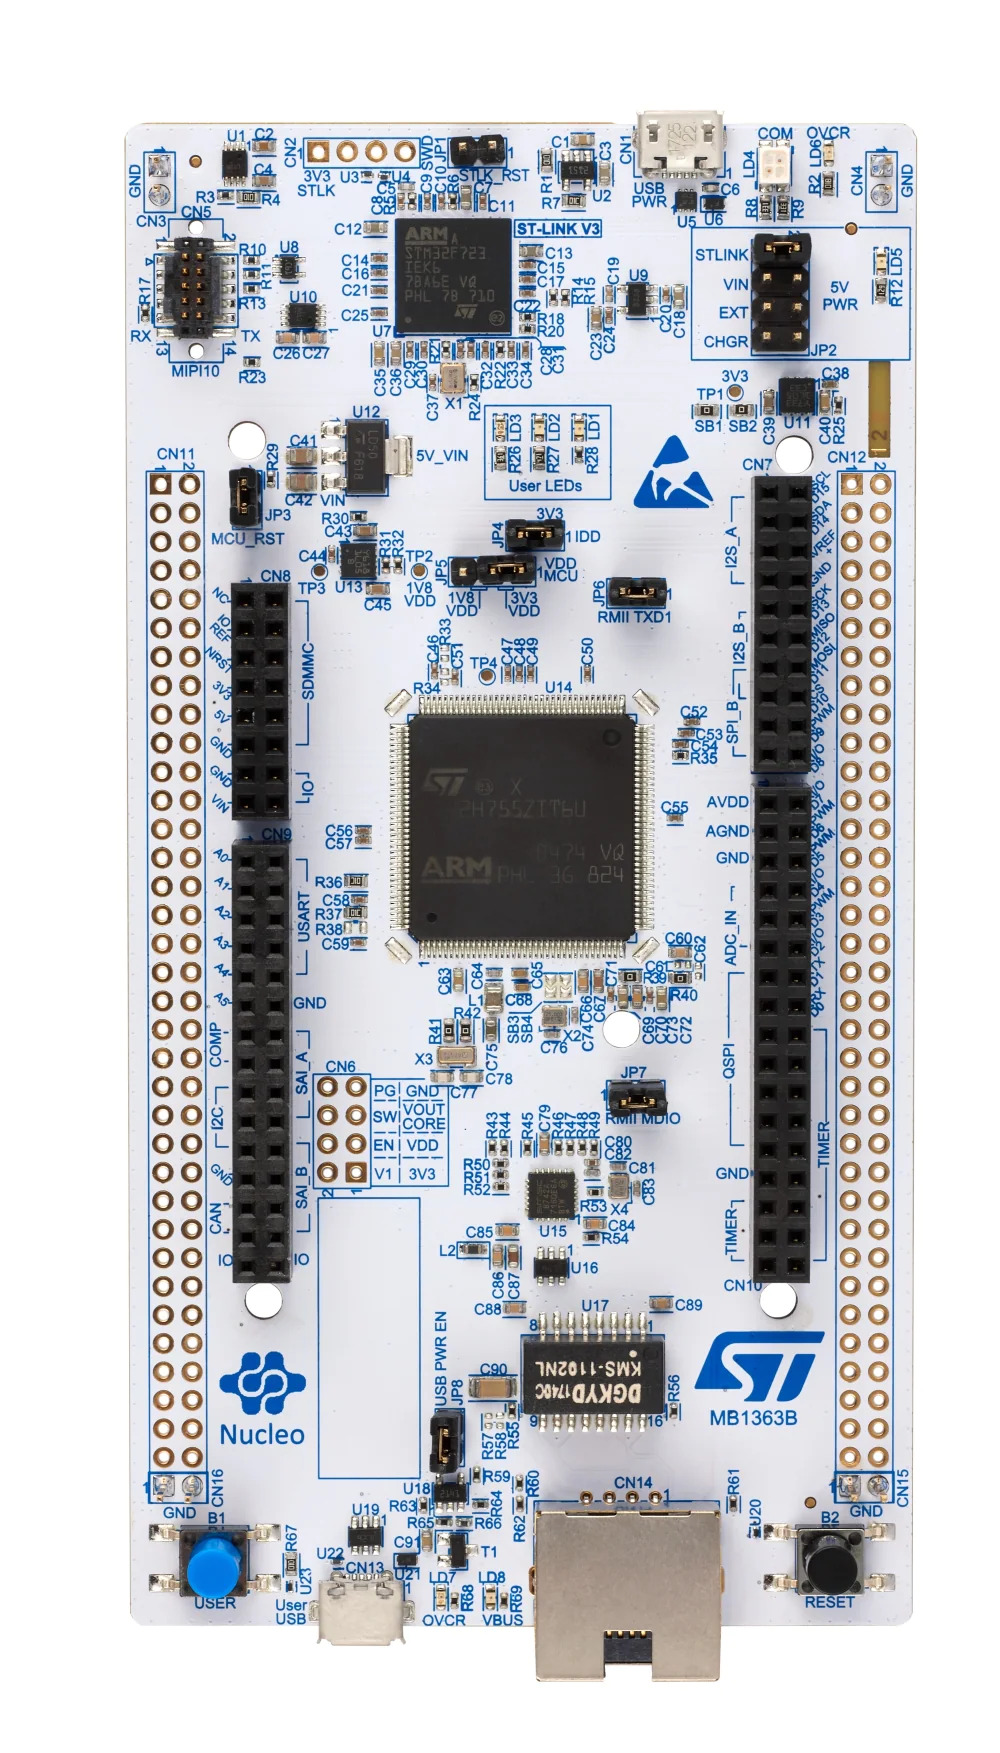
\includegraphics[height=150mm, keepaspectratio, angle=90]{figures/devboard.jpg}
    \caption{The STM32 Nucleo-H745 Development Board}
    \label{fig:Nucleo-H745}
\end{figure}

\section{Hardware Capabilities}

\subsection{Power}

Power can be provided to the MCU in a variety of ways and with different voltages ranging from 3.3 to 11 Volts. This makes it easy for developers to integrate this microcontroller into their designs. In this project, however, only the development board will be used. The easiest way to power the development board is through a micro USB port, which is also used for programming and debugging. As a connection to a PC is already needed in this early stage of development, the fact that power is also derived from this connection makes this setup comfortable to use or move.

\subsection{Clocks}

In the default setup, the MCU starts with an external clock signal that originates from the Board Management Controller. This controller is also responsible for programming and debugging. The microcontroller contains internal oscillators as well as PLLs. The usage of these can be configured in runtime during the setup phase of an application. Usually, in the first part of initializing the application the clock is set, in this case, a PLL will be used with the external clock signal from the Board Controller used as reference.

Several clock domains make it possible to fine-tune our application for low power consumption. Configuration code can be generated using official tools from the manufacturer using a GUI application. A maximum frequency of 480 MHz can be achieved for the M7 core and 240 MHz for the M4 core.

\subsection{Analog interfaces}

\subsubsection{Analog Digital Converter}

Almost all modern microcontrollers include some kind of analog-to-digital converter peripheral and the STM32H745 is not an exception \cite{ADCDescription}. It has three ADC-s where ADC1 and ADC2 are tightly coupled with ADC1 being the master while ADC3 is fully independent. Each ADC consists of a 16-bit successive approximation analog-to-digital converter and has up to 20 multiplexed channels. A/D conversion of the various channels can be performed in single, continuous, scan, or discontinuous mode. The result of the conversion is stored in a left-aligned or right-aligned 32-bit data register.

The ADC-s can use a lower resolution than 16-bit to decrease conversion time which is also independent of the AHB bus clock frequency. The ADCs are capable of self-calibration which reduces the complexity of their initialization. The start of a conversion can be initiated either by means of the software calling the applicable driver function, or hardware triggers, ie. interrupts of timer events. They are also capable of sending in interrupts themselves when a conversion is finished.

There are two main modes of using an ADC. The easiest method is using single conversion mode. With this mode, all the channel conversions are started and once these are finished, the results are stored in the appropriate registers and an end-of-conversion flag is checked. This way a blocking call to an ADC conversion can be easily implemented by waiting for the end of the conversion flag to be flipped. The second way is continuous conversion mode. Here, instead of stopping after the conversion is done and the result is placed in a register, the ADC will start this process again. When a conversion is finished it sends an interrupt that the data should be extracted from the register. Not handling this interrupt properly (ie. not saving the content of this register) will not stop the ADC from overwriting the content of the register.

The timing of a conversion can be useful information when designing an application. The elapsed time between the start of a conversion and the end of the conversion is the sum of the configured sampling time plus the successive approximation time depending on data resolution can be calculated according to the following formula.

\[T_{CONV} = T_{SMPL} + T_{SAR} = [1.5_{|min} + 7.5_{|14bit}] \times T_{adc\_ker\_ck}\]

\[ T_{CONV} = 62.5 ns_{|min} + 312.5 ns_{|14bit} = 375.0 ns\]

Where $T_{SMPL}$ is the sampling time which depends on the channel and $T_{SAR}$ depends on the resolution. In the formula above $T_{adc\_ker\_ck}$ equals 24 MHz, the resolution is 14-bit, and the lowest possible sampling time is substituted to demonstrate its usage.

\begin{figure}[H]
    \centering
    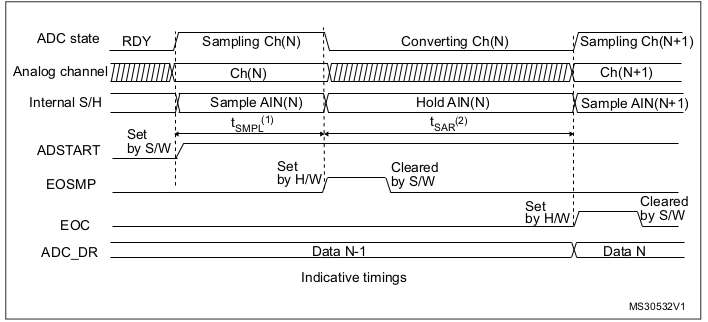
\includegraphics[width=150mm, keepaspectratio]{figures/adc-timing.png}
    \caption{Analog to Digital Conversion Timing\cite{ADConversionTime}}
    \label{fig:adc-timing}
\end{figure}

\subsubsection{Digital Analog Converter}

The DAC module is a voltage output digital-to-analog converter that can be configured in 8 or 12-bit mode. The DAC module has two output channels, and both of them have their converters. In dual DAC channel mode, conversions could be done independently or simultaneously when both channels are grouped for synchronous update operations \cite{DACDescription}.

There is one unified interface but two different DAC channels that can work in synchronized or independent modes. The DAC is able to generate noise-wave and triangular waves. They also have capabilities of using the DMA controller for their data buffers and using external triggers, ie. interrupts or timer events, for conversion is possible as well. The DAC can send interrupts to signal buffer underrun when using DMA mode but not in any other case.

When outputting a value, the DOR (Data Out Register) cannot be written directly, it should first be entered into the DHR (Data Hold Register). It is then automatically transferred to the DOR as soon as possible. This transfer is followed by a settling time which is dependent on the power supply voltage and the analog output load.

\begin{figure}[!ht]
    \centering
    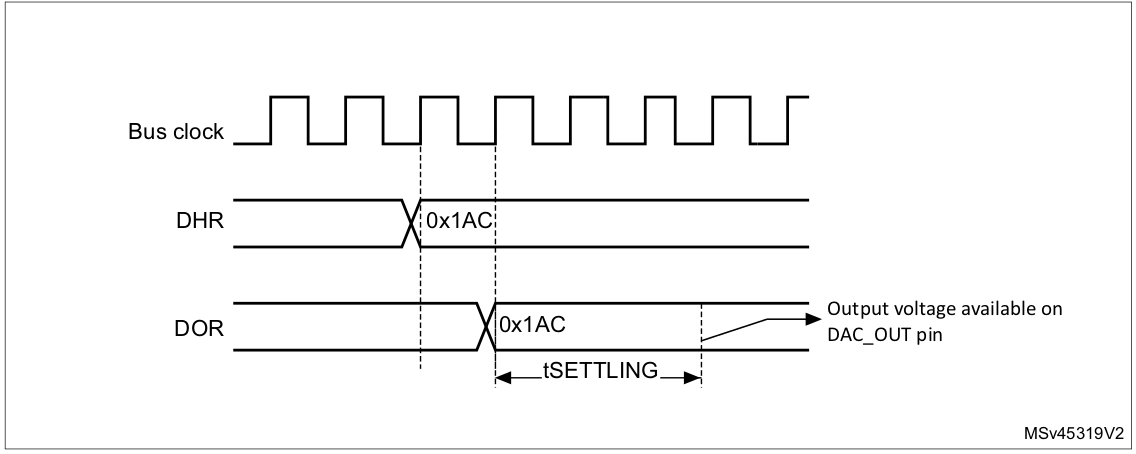
\includegraphics[width=150mm, keepaspectratio]{figures/dac-timing.png}
    \caption{Digital to Analog Conversion Timing\cite{DACTime}}
    \label{fig:dac-timing}
\end{figure}

In summary, the DAC has fewer features and fewer capabilities than the ADC on this microcontroller.

\subsection{Connectivity}

\subsubsection{Programming and debugging}

This development board is equipped with an on-board ST-LINK debugger and programmer. This module can handle the USB connection to a computer and also act as a virtual COM port or a debug port. There are multiple ways of programming the device using the ST-LINK connection, a programmer is available in the official STM IDE (Integrated Development Environment) but there are also standalone command line and GUI tools for programming. Any suitable debugger can connect to the debug port of the ST-LINK module, debugging will be described more in-depth in a further chapter.

\subsubsection{Ethernet}

Both cores of the microcontroller have pins that can be considered to use an ethernet interface. The development board has an ethernet connector that is compliant with the IEE-802.3-2002 standard. The ethernet connector is a really interesting feature for this project as in the second part when developing a more complex application. Such an application would be able to provide a minimal web GUI (Graphical User Interface) thanks to the ethernet connector.

\subsubsection{USB}

The development board has in total 2 USB Micro-AB connectors. One of them is connected to the previously mentioned ST-LINK connector so it cannot be configured freely. However, the other one is fully available for the programmer to use. Most likely this project will not utilize the USB port, but with similar complexity, and sometimes similar speeds, it could replace the ethernet port as another high-speed communication interface if needed.

\subsubsection{USART}

Multiple pins can be configured for USART peripherals, however the most important in this case is the one available through the \mycode{PD8} and \mycode{PD9} pins, which can be connected to the ST-LINK connector. By doing this we have a way of communicating with our program through a trivial communication protocol that requires minimal setup and driver support, and using the same USB port we used for powering and programming the board. Throughout development this port will be used for displaying debug traces.

\subsection{Other useful peripherals}

\subsubsection{GPIO-s}

As the pins of the STM32H745 MCU are very configurable and 144 pins are routed onto the development board, there is a considerable amount of GPIO-s that can be utilized if needed, though many of them are taken by other peripherals on the board. Three GPIO-s are each routed to a different colored user LED on the board, which is extremely useful in the early bring-up of a board as blinking an LED is often considered the "Hello World of hardware-related projects". Also present on the board are 2 buttons, one of which is a dedicated reset button while the other can be configured by the user.

\subsubsection{Hardware semaphores}

The hardware semaphore block on this system provides 32 32-bit register-based semaphores. The semaphores can be used to ensure synchronization between different processes running between different cores. They provide a non-blocking mechanism to lock semaphores in an atomic way even when multiple cores are trying to access them at the same time. There are two ways of locking one of these hardware semaphores. The first method is useful when not only the other core, but some other process from any core could try to access the semaphore. With this method, the \mycode{COREID} and \mycode{PROCID} are written to the semaphore, followed by a read check. A one-step lock is also available, where only the \mycode{COREID} is read from the semaphore.

The semaphores can generate an interrupt on any of the interrupt lines, this needs to be configured during the peripheral initialization phase. A semaphore is only cleared when \mycode{COREID} and \mycode{PROCID} match, except that a global clear is available per \mycode{COREID}. All 32 hardware semaphores have the following features: 8-bit PROCID, 4-bit COREID, 2 interrupt lines, and lock indication.

The semaphore is free when its LOCK bit is 0. In this case, the COREID and PROCID are also 0. When the LOCK bit is 1, the semaphore is locked and the COREID indicates which AHB bus master locked it. The PROCID indicates which process of that AHB (Advanced High-performance Bus) bus master locked the semaphore. When write-locking a semaphore, the COREID is taken from the master ID, and the PROCID is taken from the write data. When read locking the semaphore, the COREID is taken from the AHB bus master ID, and the PROCID is zero. There is no PROCID available with the 1-step (read) lock. The COREID is taken from the AHB bus master ID. The PROCID is written by the software of that AHB bus master. Each AHB bus master process must have a unique PROCID. PROCID is only available in the 2-step lock procedure.

\begin{figure}[!ht]
    \centering
    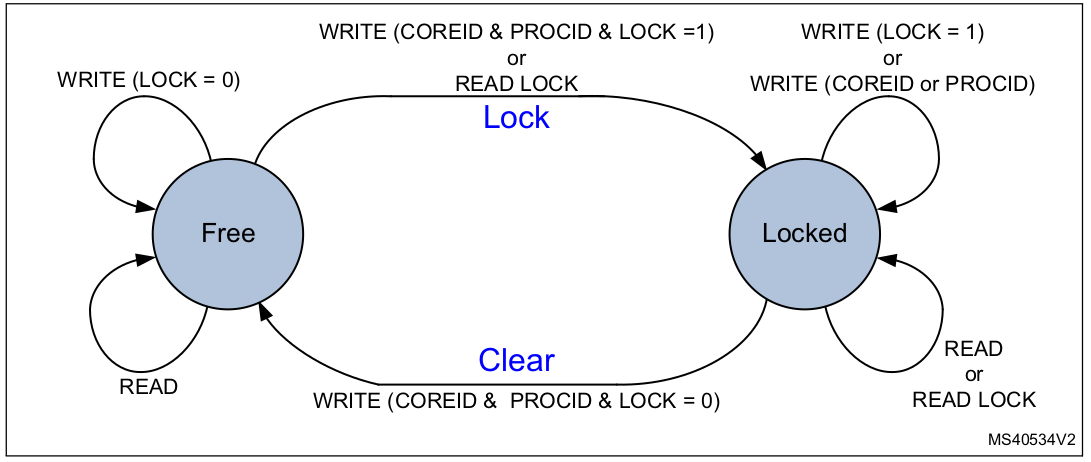
\includegraphics[width=150mm, keepaspectratio]{figures/hw-semaphore.png}
    \caption{Hardware semaphore state diagram \cite{HWSemaphore}}
    \label{fig:HWSemaphore}
\end{figure}

Clearing a semaphore is a protected process, to prevent accidental clearing by an AHB bus master or by a process that does not have the semaphore lock right. The semaphore clear procedure consists of writing to the semaphore with the corresponding COREID and PROCID and LOCK = 0. When cleared, the semaphore LOCK, the COREID, and the PROCID are all 0. When cleared, an interrupt may be generated to signal the event. To this end, the semaphore interrupt must be enabled.

\chapter{Multicore C Projects}

To create a usable multicore Rust project, a good starting point is studying C language projects created by the official tools of the manufacturer.

\section{Project Structure}

Creating C language projects for the STM32H745 microcontroller can be done in the official IDE of STMicroelectronics which is called STMCubeIDE. The software is Eclipse based and can be used to generate empty or example projects, program, and debug the code on the hardware. This is also true for multicore projects, as there are now example projects that use both cores of a H7 series microcontroller \cite{CExamples}.

Creating a dual-core project in STMCubeIDE is similar to how one would create a normal project. By selecting an H7 series MCU, not one but three connected projects are generated. A project similar to a single-core one will be created for both the M7 and the M4 core. These projects can almost function as standalone projects, they can have their source files, header files, and references. These projects also have a separate \mycode{main.c} file which contains the entry point of the current core. They also both contain builder files, linker files, and output folders, so essentially they can be built separately. By default, programming and debugging are also done with these separate projects, so when the IDE is used the cores are programmed one by one. Also as a limitation of the software, only one of the two cores can be effectively debugged at a time, while the other one either runs or is in a HALT state.

The project is a wrapper for the previous two that rests above them in a hierarchical sense. It can also contain common code that can be referenced and shared from the core-specific projects. Most of the drivers can reside in this project, as regarding peripherals, the M7 and M4 cores are similar. The wrapper project also contains parts of the code that directly refer to dual-core functionalities, for example, definitions of some memory locations and even some code regarding dual-core boot can be found there.

In STM32 projects, lots of code around setting up the peripherals is generated during project creation. This is no different in a dual-core project. Setting the function of each pin of the MCU can be done with a GUI, which then generates the code that will configure those pins correctly. The peripherals can be further configured in this GUI by enabling them, an initialization code will be added to the \mycode{main.c} source file of one of the core-specific projects. In dual-core projects, the core that initializes a peripheral can be selected separately for each one, while also allowing both cores to use the same peripherals when one is enabled for both of them.

Besides the pinout configuration, the clock configuration can also be set in this GUI. This is especially helpful if our project requires different clocks for different clock domains. The clock settings can be configured in a hierarchical graphical interface where the sources and multiplications are visualized on a flow-control diagram. Clock signals for certain domains can even be turned off to save power if none of the corresponding peripherals are used.

\section{An Example Project}

To fully understand the intended use of this dual-core MCU, we must take a look at a simple example project. This will give us a clear picture of how the microcontroller starts, how peripherals are handled, and how the two cores communicate. The project this essay will take a closer look at is an example project from ST that uses message buffers from FreeRTOS to demonstrate communication between the two cores \cite{CDemo}.

\subsection{General description}

After the initialization phase, the M7 core will send data using message buffers. The data will be received by the M4 core which is not using an RTOS but running a bare metal application, though the FreeRTOS header will still need to be included to have access to its message buffer type. There is no communication in the other direction. This communication requires that the message buffer is declared in a shared memory which is accessible to both cores. Additionally, the address of the buffer must be known to be the same at compile time for both cores. The data received by the M4 core will be checked for correctness, and if found correct, LED1 will be toggled. In case of an error, LED2 will be set and the M4 core will enter an empty infinite loop. This operation takes place every 500 milliseconds. While M4 core busy waits for data in the message buffer the M7 core only sends the data after a 500 millisecond delay in every iteration.

\subsection{Initialization phase}

The initialization of the M4 core is more trivial than that of the M7 as the M4 handles the setup of the peripherals used. This is usually the case in these types of projects, and it is a good practice to have a controller core that can control peripherals and event the other core in the early stages of the application.

Firstly, the L1 data and instruction cache are enabled for the M7 core. The dangers of using a non-shared cache should be kept in mind when creating projects that implement communication between the cores. The obvious solution is to invalidate the cache before reading or writing data to shared memory addresses, however, on this MCU another, more convenient solution is also possible and used in this example. The next step is configuring the MPU (Memory Protection Unit). This peripheral, if set up correctly, can ensure correct cache contents by setting some regions of memory as non-cachable. The MPU can be configured using an MPU initialization struct. Its most important fields in this example are \mycode{IsCacheable} and \mycode{IsShareable}, and of course, the selected region must also be given in this struct. The shared variables will be located in the \mycode{D3\_SRAM} so it is set to be non-cachable and shareable in this example.

While this is happening, the M4 core also starts and as it lacks cache and the MPU is handled by the other core, it starts to initialize its own variables and a hardware semaphore that will be used for inter-core communication. After that, the M4 core puts itself into deep sleep mode, to wait for the other core while it finishes the initialization of the common peripherals.

After configuring the MPU and its own cache the M7 core will busy wait for the M4 core to go into a deep sleep state by continuously reading a register that stores information about the clock domain of the other core. When the other core is properly HALT-ed, the M7 can continue with the initialization of peripherals used by both cores. It will first setup the Hardware Abstraction Layer system, then will go on to initialize the clock system. In this case, the frequency is set to 400 MHz and half of that for the M4 core, but this part of the code is generated based on the GUI settings described already.

Finally, the message buffer is created on the M7 core, and the M4 core can be released from the sleep state. The M7 core will enable the clock of the domain where the previously mentioned hardware semaphore is located, then takes and releases the semaphore to wake up the other core. After this, a FreeRTOS task is created and the scheduler is started. After waking up, the M4 core will initialize the 2 LEDs it will use and enters into its infinite loop.

\subsection{Running phase}

There is only one task scheduled to run on the M7 core. This task simply creates a string that contains a number that is incremented after every iteration. This number is then placed into the message buffer and the task requests a 500 ms delay. This is the time the other core has for reading the value, as after this the buffer is reset by the M7 core. The M4 core starts with creating a string in local memory which will be compared to the one received, by having a similar local counter that gets incremented after every read from the buffer. After this, the M4 core busy waits until some data is placed in the message buffer, and immediately reads it once it arrives. It then compares it to the locally created string and if the values match, it toggles LED1 and if they do not, it goes into an error handler function. This function turns off LED1 and turns on LED2 to signal the error, then goes into an empty infinite loop. This loop of course could be modified to handle the error, but that is out of the scope of this study.

\chapter{Multicore Rust Project}

Before any application can be developed in Rust for this MCU, the state of Rust support needs to be properly assessed for both single and dual core STM32H7 devices. By the end of this chapter, a multi core Rust "Hello World" project should be ready as a starting point for more complex applications.

\section{Single core support}

\subsection{General structure}

As mentioned before, STM32 hardware has a relatively strong Rust support regarding MCU-s and their peripherals, even the development boards in some cases. But the typical project structure is very different from what was discussed in the previous chapter about C projects and using STMCubeIDE. The Rust crates that support embedded devices are layered hierarchically, first there is a crate required for every Cortex-M microcontroller: \mycode(cortex-m), then the \mycode{embedded-hal} crate expands upon that with functionalities commonly found in HAL drivers. Below that is a crate called \mycode{stm32-hal}, which is then expended upon by \mycode{stm32h7xx-hal} which can finally be used on the STM32H745 microcontroller, sadly with the twist that only the M7 core will function properly without doing some kind of workaround. Though not an official crate by ST there exists a BSP crate for the development board used in this project called \mycode{nucleo-h7xx}. This crate provides useful abstractions over the previous crate in the dependency chain, but as it will be discussed later, using this BSP crate would only complicate things in the long run for this project.

It is also worth mentioning that the \mycode{stm32h7xx-hal} crate depends on another crate called \mycode{stm32h7}. This crate provides type safe access to the peripherals of H7 series ST microcontrollers. These type of projects generate their register maps from SVD files using the \mycode{svd2rust} tool. The tool is maintained by the developers of the Rust language and is used extensively when creating support for a new embedded device.

\subsection{An embedded Rust project}

Rust projects are fairly lightweight compared to projects generated from some IDE like STMCubeIDE. For example here is the structure of a new project generated by the \mycode{cargo init} command.

\begin{lstlisting}[language=C,frame=single,float=!ht,label={lst:rust-project-structure},caption={Rust Project Structure}]
    .
    |-- Cargo.toml
    |-- src
        |-- main.rs

\end{lstlisting}

Essentially only 2 files were created. \mycode{Cargo.toml} will hold information about the project, such as its name and version, but it will also list all the dependencies. Build targets can also be defined in this file, it basically fills the role of a "project setting" or "project properties" window from an IDE. This file can be modified by hand and the changes will take effect on the next compilation, but some cargo commands will also modify it automatically. For example a dependency can be added by listing it under the \mycode{[dependencies]} section header and building the project, or by running the \mycode{cargo add <crate>} command, which will automatically list the dependency in the file. Some features can also be defined for these dependencies, the main one being their minimum required version, but soon some other ones will become important when the STM32 related crated will be added.

The other file is the \mycode{main.rs} source file that contains the entry point of the program, a main function. By default, this file contains a basic "Hello World" program, so the project can already be built and ran.

\begin{lstlisting}[language=C,frame=single,float=!ht,label={lst:rust-hello-world},caption={Rust Hello World Porgram}]
    fn main() {
        println!("Hello, world!");
    }
\end{lstlisting}

Of course this basic project is not going to work on a microcontroller without some major changes. Here are the necessary steps that need to be taken before a new Rust project produces a binary that can be loaded onto an MCU.

When we installed the Rust toolchain on a computer, it automatically detected the CPU-s architecture, and fledged a compiler specific to that. To compile to another architecture, we need to add another target to our toolchain. This can be done with the command \mycode{rustup target install thumbv7em-none-eabihf} which installs a compiler that can target ARM Cortex-M cores with floating point support. The target depends on the capabilities of the microcontroller, but in case of this project, both cores of the STM32H745 can use this toolchain.

A way to program the microcontroller is also needed. A Rust native tool is cargo-flash which can be installed with \mycode{cargo install cargo-flash}. It automatically detects how to program a microcontroller based on its type if it is supported. However once the project was built, any other way can be used to program the MCU. Further on, I will talk about challenges around programming this specific device.

Once our toolchain was expanded with the previous tools, we need to modify the basic project to use these tools. A new configuration file \mycode{.cargo/config} should be created. This is also a TOML file that configures the project, but instead of storing dependencies and higher level concepts, it will relate directly to the compilation phase. The new file will contain a line which selects the previously added target as the default one when building. Information about the linking phase can also be supplied here for example, in the \mycode{cortex-m} crate there is a linker script \mycode{link.x} which needs to be explicitly included in every project that uses this, or any other crate using it. Many other tweaks can be configured in this file, but these two are necessary for building a minimal working program. Here is a sample file that contains these two configurations.

\begin{lstlisting}[language=C,frame=single,float=!ht,label={lst:cargo-config-file},caption={Cargo Config File}]
    [build]
    target    = "thumbv7m-none-eabihf"
    rustflags = [ "-C", "link-arg=-Tlink.x" ]
\end{lstlisting}

Of course the basic linker script from will not be enough, a linker script specific to the MCU we intend to use must also be supplied. This can be done by creating a file called \mycode{memory.x} at the root of the project, and filling it with information about the memory mapping of the selected microcontroller. However in this case the linker script is already part of the \mycode{stm32h7xx-hal} crate, so it does not need to be created manually if we plan to use this crate.

With that done, we will need to add some necessary dependencies. As a \mycode{memory.x} linker script was not created manually, we must include the \mycode{stm32h7xx-hal} under as a dependency. Besides its minimal version, a feature set also needs to be specified here for this crate to work properly. Another necessity was already mentioned before, a panic handler needs to be created as any code can panic unexpectedly, and the program cannot quit without an underlying operating system. \mycode{panic-halt} is a crate that adds a default panic handler that puts the processor into a HALT state when the program running on it panics. So a working project for the M7 core should contain at least the following contents in its \mycode{Cargo.toml} file.

\begin{lstlisting}[language=C,frame=single,float=!ht,label={lst:cargo-toml},caption={Cargo.toml File of the Project}]
    [package]
    name = "blink"
    version = "0.1.0"
    edition = "2021"

    [dependencies]
    cortex-m = "0.7.7"
    cortex-m-rt = "0.7.3"
    panic-halt = "0.2.0"
    stm32h7xx-hal = {version = "0.14.0", features = ["stm32h747cm7"]}
\end{lstlisting}

The only thing left after this is writing valid code that does something, such as blinking an onboard LED. Notice that there was no step that involved code generation based on GUI tools as was the case in STMCubeIDE. This means that all configurations will need te be done directly in the code, which can sound scary, but the rich types and strict compiler of Rust will help us make sure that the hardware passes the smoke test when we turn it on for the first time.

The first step of writing embedded code is getting rid of the standard library crate and the traditional main function with the \mycode{#![no_std]} and \mycode{#![no_main]} directives. Of course the program will still need an entry point, and that is why the \mycode{cortex-m-rt} crate is included in the project. This crate provides the \mycode{#[entry]} directive that can mark a function as the entry point of the program. It can still be called main, but is must have the following signature.

\begin{lstlisting}[language=C,frame=single,float=!ht,label={lst:embedded-main},caption={Main Function in Embedded Rust}]
    #[entry]
    fn main() -> ! {
        loop {}
    }
\end{lstlisting}

This code snippet describes main as a function that takes no arguments and does not return at all. This is why only a loop is present in its body, the loop expression is a shorthand for an infinite loop in Rust.

To make a simple blinking program only two more things are required. First we need to have some method to measure the time between the toggles of an LED, then a function that can actually toggle the LED. The \mycode{cortex-m} crate contains a \mycode{delay\_ms()} function that will insert the appropriate amount of NOP assembly statements to the code to wait at least the specified amount of milliseconds. Interrupts and a timer peripheral could also be used, but at this point we only aim to create a minimal working application and using busy waits is much easier. For the LED-s to work we just need to take the \mycode{GPIOE} peripheral and split it into a structure of pins. Then we take the \mycode{pe1} pin, configure it into push-pull mode and it can be controlled with the \mycode{set\_high()} and \mycode{set\_high()} functions.

\begin{lstlisting}[language=C,frame=single,float=!ht,label={lst:embedded-hello-world},caption={Embedded Hello World (Blink) in Rust}]
#![no_main]
#![no_std]

use cortex_m_rt::entry;
use stm32h7xx_hal::{pac, prelude::*};
use panic_halt as _;

#[entry]
    fn main() -> ! {
        let cp = cortex_m::Peripherals::take().unwrap();
        let dp = pac::Peripherals::take().unwrap();

        let pwr = dp.PWR.constrain();
        let pwrcfg = pwr.freeze();

        let rcc = dp.RCC.constrain();
        let ccdr = rcc.sys_ck(100.MHz()).freeze(pwrcfg, &dp.SYSCFG);

        let gpioe = dp.GPIOE.split(ccdr.peripheral.GPIOE);

        // Configure PE1 as output.
        let mut led = gpioe.pe1.into_push_pull_output();

        // Get the delay provider.
        let mut delay = cp.SYST.delay(ccdr.clocks);

        loop {
            led.set_high();
            delay.delay_ms(500_u16);

            led.set_low();
            delay.delay_ms(500_u16);
        }

    }
\end{lstlisting}

One main difference in Rust compared to C is that peripherals are objects and can only be created or taken in a certain way instead of just creating a variable with the appropriate type. For example, we are forced to set power constraints to be able to set the system clock to a frequency, which in turn is needed to access the GPIO-s. Both the peripherals from the \mycode{cortex-m} and the \mycode{stm32h7xx-hal} crate are part of a singleton module. This is done deliberately so they are not taken more times than one by accident, which is very useful for single core applications, but may become bothersome with multicore usage. This is of course an open issue with the \mycode{cortex-m} crate and is yet to be assessed. \cite{MulticorePeripherals}

With all this, a simple, single core application is ready and we can start to research how it can be made to accommodate code for the other core. Loading the application is possible with the previously mentioned \mycode{cargo-flash} tool, though it will not be able to figure out the chip type, it can supplied as an argument.

\begin{lstlisting}[language=C,frame=single,float=!ht,label={lst:cargo-flash-1},caption={Flashing the Image with Cargo Flash}]
    cargo flash --chip STM32H745ZITx
\end{lstlisting}

\section{Multicore project structure}

This section discusses possible structures and hierarchies for a multicore project in Rust for the STM32H745 microcontroller.

\subsection{Separate projects for cores}

The first idea of a multicore project is to copy the structure of multicore C setup as closely as possible. This solution would require two completely separate projects for the two cores which would allow for great flexibility as the code would be loosely coupled between cores. Developing independent applications for the two cores would be the most comfortable this way. However a way for the two cores to communicate must also be included in a project like this, and that is most commonly done using some sort of shared memory. Defining shared memory sections requires the connection of the two projects on some level at least in the linking phase of compilation. As of writing this part of the essay, no project structured like this could be found that could support all the necessary features. This means that if this method of project organization is selected, besides making an example application, a framework also needs to be created to support the structure. This would not be impossible but would be questionable if it would fit into the time frame of the project, so it necessary to explore other ways of creating a multicore project structure.

\subsection{Single project for all cores}

At the other end of the spectrum, it is possible to compile code for both cores from a single project by modifying the linker script. This could be achieved by defining the entry point of the second core and and placing its code in the correct memory segment using the \mycode{memory.x} linker script. The advantage of this method over the previous one is that shared memory is easily defined and handled as there will not be separate compilation and linking for the two cores, it will be done in one go. There are also drawbacks however, for example the two cores can ever only use the same crates, as there is only one project so its dependencies cannot be changed for each core. On top of this, the usage of peripherals will run into the same problem discussed earlier. As the peripherals form a singleton module and there is only a way to "take" them but no way to "give" them, only one core will be able to access them safely. Finding a workaround for this issue without compromising safety is also a task that may run out of the time frame of the project.

Despite the drawbacks, one more advantage is that there is a very low level example project using this project structure from a prominent member of the embedded Rust community. \cite{DualCoreDemo} This example project does not use the \mycode{stm32h7xx-hal} crate get access to the peripherals but rather a crate called \mycode{stm32-ral}. This register access layer crate provides access to the peripheral registers of the microcontroller, so it circumvents the singleton limitation of HAL crates. However using this crate for a bigger project may not be feasible as more complex peripherals, for example the ethernet connector, can be difficult to use without drivers and only using the peripheral registers.

During this research, a half solution was found for this obstacle. By using both the \mycode{stm32h7xx-hal} and the \mycode{stm32-ral} crates, both cores can have access to the peripherals. The M7 core would use the HAL crate and the M4 core would use the registers to access the peripherals. This would introduce a limitation into further application development, as drivers would only be available for the M7 core. Still, the M4 core could access peripherals, and handling the less complex ones could be done using registers, while the M7 core would use the more complex ones with proper HAL drivers.

To create this project, we need to update the \mycode{Cargo.toml}, \mycode{memory.x} and \mycode{main.rs} files. \mycode{Cargo.toml} will receive the following line in its dependencies section.

\begin{lstlisting}[language=C,frame=single,float=!ht,label={lst:stm32-ral},caption={STM32 RAL in Cargo.toml}]
    stm32ral = { version = "0.8", features = ["stm32h747cm4"], default-features = false }
\end{lstlisting}

Notice that while the \mycode{stm32h7xx-hal} crate was added with \mycode{stm32h747cm7} features, the register access layer is added with \mycode{stm32h747cm4} features, as it will be used by the M4 core. The linker file will also needs to be modified, which means that is needs to be copied out from the HAL crate and included in our project as a file so it can be edited. Besides the default definitions in this file we need to define the stack, reset table and vector table for the second core. The flash area for the second core is already defined in the script, so as an extension we just need to populate it with the correct code. The stack of the second core can be defined as follows. For reference, the definition of the stack for the first core is also presented.

\begin{lstlisting}[language=C,frame=single,float=!ht,label={lst:link-starts},caption={Stack Definitions in Linker File}]
    _stack_start = ORIGIN(RAM) + LENGTH(RAM);
    _cpu2_stack_start = ORIGIN(SRAM2) + LENGTH(SRAM2);
\end{lstlisting}

To make sure that the reset and vector tables of the second core will be at the correct parts of the flash, the following code can be added to the \mycode{SECTIONS} block of the linker script.

\begin{lstlisting}[language=C,frame=single,float=!ht,label={lst:link-flash2},caption={Flash Definition of Second Core in Linker File}]
    .flash2 : ALIGN(4) {
        LONG(_cpu2_stack_start);
        KEEP(*(.flash2.reset_vector));
        KEEP(*(.flash2.vector_table));
        *(.flash2 .flash2.*);
        . = ALIGN(4);
    } > FLASH2
\end{lstlisting}

Finally, a main function can be created for the second core.

\begin{lstlisting}[language=C,frame=single,float=!ht,label={lst:embedded-main2},caption={Main Function of Second Core}]
    unsafe extern "C" fn main2() -> ! {
    write_reg!(rcc, RCC, AHB4ENR, GPIOBEN: Enabled);
    write_reg!(gpio, GPIOB, MODER, MODER0: Output, MODER14: Output);
    write_reg!(gpio, GPIOB, ODR, 0);
    loop {
        write_reg!(gpio, GPIOB, BSRR, BS0: 1);
        cortex_m::asm::delay(4_000_000);
        write_reg!(gpio, GPIOB, BSRR, BR0: 1);
        cortex_m::asm::delay(4_000_000);
    }
}

#[no_mangle]
#[link_section=".flash2.reset_vector"]
pub static CPU2_RESET_VECTOR: unsafe extern "C" fn() -> ! = main2;
\end{lstlisting}

The function itself initializes a GPIO and its clock, then toggles it every 4 million CPU cycles. The actual time of the delay will be determined by the frequency configured by the other core. Below the function the directives can be seen that will place the address of this function in the reset vector for the M4 core. While this solution could work well, there are some compromises, so it is worth investigating further in hopes of finding a better project structure.

\section{The microamp framework}

The microamp framework was developed recently as a framework for multicore embedded devices. It sort of combines the previous two approaches by providing a way to compile different codes for the two cores, but retaining the possibility of placing variables in shared memory. The framework provides two main functionalities. One of them is the \mycode{#[shared]} attribute, which can signal that a variable should be placed in shared memory. This also requires that some parts of the memory map must be marked as shared in the linker script, and the variable must also be static. The other main functionality is code sharing and division between the cores. By default, every code will be compiled and loaded onto both cores. However with attributes such as \mycode{#[cfg(core = "0")]} or the \mycode{cfg!(core = "0")} macro parts of the code can be directed to only be compiled to a specific core.

\subsection{Shared variables}

As already stated, shared variables can be declared the following way.

\begin{lstlisting}[language=C,frame=single,float=!ht,label={lst:shared-variable},caption={Shared Variable Example}]
    #[shared]
    static mut SHARED_VAR: u32 = 0;
\end{lstlisting}

The attribute does not affect the compile process directly as this variable will be present in the binary output for both cores, but possibly on different memory addresses. However here is where the microamp framework comes in. After the compilation of the first core is done the location of any variable marked as shared will be stored, and during the building of the second core binary, these location of these variables can be set to match the addresses found in the first image.

One thing to be aware of with shared variables that are defined this way is that their initial value is only written in memory during the flashing process. Warm or even cold resetting the microcontroller will not set these variables back to their initial values. This is an unintended consequence of optimizations by the compiler. The rest of the optimizations are useful for the project thus turning them off would not be beneficial in the long run. The easy fix to this issue is adding a line which sets this variable to the default value.

\begin{lstlisting}[language=C,frame=single,float=!ht,label={lst:shared-variable2},caption={Shared Variable Example With Default Value}]
    #[shared]
    static mut SHARED_VAR: u32 = 0;
    unsafe { SHARED_VAR = 0; }
\end{lstlisting}

Of course this default value can be assigned at other places of the code and most of the time only one of the cores need to set it.

As it can be seen in Listing~\ref{lst:share-variable2} accessing these variables from any core is obviously an unsafe action so rust forbids it outside of code blocks marked \mycode{unsafe}. We usually need unsafe blocks to directly access memory anyway, that does not mean these accesses cannot be made safe, it just means that the potential of memory access violations or data races are present, and the programmer should take extra care with these parts of the code. In the case of a single shared variable a semaphore would suffice for making its access safe. Ideally, a hardware semaphore should be used, but for the first proof-of-concept project, the \mycode{AtomicU8} type will work in almost all cases. The only time a software semaphore cannot work correctly is if the two cores request access in the same clock cycle. For a real embedded device that margin of error is not good enough, but for this example, it will work fine.

First, we have to declare another shared variable.

\begin{lstlisting}[language=C,frame=single,float=!ht,label={lst:sw-semaphore1},caption={Software Semaphore Variables}]
    const CORE0: u8 = 0;
    const CORE1: u8 = 1;
    const LOCKED: u8 = 2;

    #[shared]
    static SEMAPHORE: AtomicU8 = AtomicU8::new(CORE0);
\end{lstlisting}

Some constants are also defined to make the example easier to understand. Next, two constant variables are created, but the value of them will differ based on which core we are currently compiling for.

\begin{lstlisting}[language=C,frame=single,float=!ht,label={lst:sw-semaphore2},caption={Software Semaphore Core Specific Variables}]
    let (our_turn, next_core) = if cfg!(core = "0") {
        (CORE0, CORE1)
    } else {
        (CORE1, CORE0)
    };
\end{lstlisting}

With these variables the semaphore can now be locked and unlocked. Unlocking automatically gives the resource to the other core.

\begin{lstlisting}[language=C,frame=single,float=!ht,label={lst:sw-semaphore3},caption={Software Semaphore Locking and Unlocking}]
    while SEMAPHORE
        .compare_exchange(our_turn, LOCKED, Ordering::AcqRel, Ordering::Relaxed)
        .is_err()
    {
        // Busy wait if the lock is held by the other core
    }

    // Release the semaphore
    SEMAPHORE.store(next_core, Ordering::Release);
\end{lstlisting}

To protect a resource a simple mutex can be created. The mutex is enforced by a shared variable similar to the previously described semaphore. The resource guarded with this variable can be accessed by the same core multiple times in a row.

\begin{lstlisting}[language=C,frame=single,float=!ht,label={lst:sw-mutex1},caption={Mutex For a Variable}]
    const UNLOCKED: u8 = 0;
    const LOCKED: u8 = 1;

    #[shared]
    static mut CURRENT_VOLTAGE: f32 = 0.0;

    #[shared]
    static MUTEX: AtomicU8 = AtomicU8::new(UNLOCKED);
\end{lstlisting}

\begin{lstlisting}[language=C,frame=single,float=!ht,label={lst:sw-mutex2},caption={Performing a Read Operation Using a Mutex}]
    while MUTEX
    .compare_exchange(UNLOCKED, LOCKED, Ordering::AcqRel, Ordering::Relaxed)
    .is_err()
    {}

    // MUTEX TAKEN
    let display_voltage;
    unsafe {
        display_voltage = CURRENT_VOLTAGE;
    }

    MUTEX.store(UNLOCKED, Ordering::Release);
    // MUTEX GIVEN
\end{lstlisting}

\subsection{Divergent code}

It is not a strange thing in Rust that compile time directives look similar to "active code" that will actually be translated to machine instructions. This is by design so the code becomes readable on a higher level, however makes the language harder to understand when dealing with low level compilation tasks. In this example project the infinite loop of the application will be fully different for the two cores.

\begin{lstlisting}[language=C,frame=single,float=!ht,label={lst:divergent-code},caption={Example of Diverging Code}]
    loop {
        match () {
            #[cfg(core = "0")]
            () => {
                writeln!(tx, "Hello World!\r\n").unwrap();
                while SEMAPHORE
                    .compare_exchange(our_turn, LOCKED, Ordering::AcqRel, Ordering::Relaxed)
                    .is_err() {}
                unsafe {if SHARED > 5 {delay_time = 1000_u16}}
                SEMAPHORE.store(next_core, Ordering::Release);
                led.set_high();
                delay.delay_ms(delay_time);

                led.set_low();
                delay.delay_ms(delay_time);
            }
            #[cfg(not(core = "0"))]
            () => {
                while SEMAPHORE
                    .compare_exchange(our_turn, LOCKED, Ordering::AcqRel, Ordering::Relaxed)
                    .is_err() {}
                unsafe {SHARED += 1;}
                SEMAPHORE.store(next_core, Ordering::Release);
                led2.set_high();
                delay.delay_ms(500_u16);

                led2.set_low();
                delay.delay_ms(500_u16);
            }
        }
    }
\end{lstlisting}

When this code is compiled, the M7 core will only contain the upper arm of the match expression and the M4 will get the lower arm. In this example program one LED is continually toggled by the M7 core, while another one is toggled by the M4 core. The M4 core increments the shared variable by one in every iteration, while the other core reads it every time. After 5 cycles of this, the blinking speed of the LED operated by the M7 core is reduced by a factor of 4. This indicates that the variable can be written by one of the cores and written by the other.

The first part of this code is the same for both cores, which in turn is the same as the code in the single core case. Both cores create an instance of the singleton peripherals, so they both can have unrestricted access. This is another area where data races need to be prevented by the programmer. In this case the cores never use the same GPIO port, the LED-s are operated are located on separate ones, but in the future, if the two cores do need to use the same peripheral, they will also need to be protected by a semaphore, ideally a hardware semaphore.

\section{Linker scripts}

There is one more thing missing for the dual-core program to function properly. The microamp framework requires a separate linker script called \mycode{core0.x}, \mycode{core1.x} etc., one for every core. This presents another problem for this project. The \mycode{link.x} linker script from the \mycode{embedded-hal} crate is special in the sense that it wants to include a linker file called \mycode{memory.x}. In simple cases this is not an issue as HAL crates usually provide this file and if not, we can create it in the root of our project. However the microamp framework does not require this the \mycode{memory.x} script, but separate ones like \mycode{core0.x}, which usually hold almost the same content as the \mycode{memory.x} script just a bit more customized for the specific core.

So the problem is that \mycode{link.x} requires a single \mycode{memory.x}, but we have \mycode{core0.x} and \mycode{core1.x} which hold similar content but differ in some places. For example, the \mycode{stm32h7xx-hal} crate requires that a \mycode{RAM} and a \mycode{FLASH} symbol is defined in one of the linker scripts of the project. However exactly these symbols need to differ for the two cores, so this definition cannot be at a common place.

The workaround this issue is as follows. In both \mycode{core0.x} and \mycode{core1.x} the memory and the \mycode{RAM} and \mycode{FLASH} symbols are defined at the start of the linker script. The memory map is taken directly from the \mycode{memory.x} file of the HAL crate. After these are defined, the \mycode{link.x} script can be included so it is part of the build process. This means that is can be removed from the \mycode{.cargo/config} file. As we know, the \mycode{link.x} script will try to include a \mycode{memory.x} file so it needs to exist, but cannot and does not need to hold any information, so in my case it is just an empty file. The rest of the core specific linker scripts is \mycode{SECTIONS} block which only differs at the very end where the reset and interrupt vectors are defined, as we have to make sure those go to the correct flashes.

The last thing we need to do is define a memory section that can be used as a shared memory. For this demonstration the \mycode{AXISRAM} memory was chosen. Both cores have read and write access to it so it can serve this purpose. The following lines should be added in the \mycode{SECTIONS} block to define the shared memory.

\begin{lstlisting}[language=C,frame=single,float=!ht,label={lst:link-shared},caption={Defining Shared Memory in Linker File}]
    .shared : ALIGN(8) {
        KEEP(microamp-data.o(.shared));
        . = ALIGN(8);
    } > AXISRAM
\end{lstlisting}

\section{Build flow}

The microamp framework is in alpha state so it requires the nightly version of the rust toolchain. Besides that, building the project is pretty simple using the \mycode{microamp} command.

\begin{lstlisting}[language=C,frame=single,float=!ht,label={lst:cargo-microamp},caption={Building a Dual Core Application with Microamp}]
    cargo +nightly microamp --bin blink --release
\end{lstlisting}

\section{Flashing}

Loading the program onto the MCU is no longer the most convenient using \mycode{cargo-flash} as we now have two binaries after a single build. Images that contain the code for one or both of the cores can be flashed into the MCU using an official GUI tool from ST called CubeProgrammer. Before flashing a tool called \mycode{srec_cat} is used to create a single image from the two core specific outputs. The unified image can then be flashed using the CubeProgrammer program. For a more automated flashing process, ST provides a command line utility called \mycode{st-flash} which is part of the STLink Tools program package /cite{STLinkTools}. However this program runs into an error when a flashing an image that covers the memory region of both cores. This error \cite{STFlashError} is already well documented and its fix will be the part of the next release cycle. Until then the STMCubeProgrammer GUI tool remains the most efficient way of loading our programs onto the microcontroller.

\chapter{Improvements to the Basic Project}

In the previous chapter, the focus was on creating a project that can target a dual-core STM32 microcontroller. It was however only a basic "Hello World" type project that can be massively improved upon. In this chapter, I will demonstrate the steps that were taken before attempting to build a proper example project.

\section{UART}

Establishing a serial connection between the target MCU and the host PC is usually the most important first step at the start of a new embedded project. While a UART line may not have full debugging capabilities, it allows for quick and relatively easy text-based communication with the host. These traces are a very effective tool in determining where a program gets stuck in a loop or panics.

The following code brings up the UART interface that is linked to the ST-Link connector on the board. In this project, this UART interface is used for debugging purposes, so only the rx line is not in use. Rust generates warnings for variables that are not used, this can be avoided by prepending an underscore to the unused variable. The serial line is configured to operate with 19200 baudrate and without flow control.

\begin{lstlisting}[language=Rust,frame=single,float=!ht,style=customrust,label={lst:uart-bringup},caption={UART Interface Configuration}]
    let tx = gpiod.pd8.into_alternate();
    let _rx = gpiod.pd9.into_alternate();
    let serial = dp
        .USART3
        .serial((tx, _rx), 19200.bps(), ccdr.peripheral.USART3, &ccdr.clocks)
        .unwrap();
    let (mut tx, _rx) = serial.split();
\end{lstlisting}

\section{Debugger}

Using traces on a serial line for detecting errors in the code may not be sufficient in all cases. Moreover, the overhead of printing to this peripheral can disrupt the timing of certain parts of the program. In these cases configuring a debugger becomes a necessity.

All STM32 development boards are equipped with an on-board ST-Link debugger. ST-Link connects to the host PC through a USB interface. The ST-Link can facilitate debugging through different modes of communication for example single-wire interface module (SWIM), serial wire debugging (SWD), and Joint Test Action Group (JTAG) of which the latter is used most often.

The official IDE provided by STM, STMCubeIDE includes full debugging capabilities, however, these tools can only handle C and C++ code. The Rust ecosystem does not currently have a standard tool nor does STM provide debugging tools for other languages. Most often though Rust developers will use openocd, gdb, and VSCode.

\subsection{OpenOCD}

Open On-Chip Debugger (OpenOCD) is an open-source tool that provides debugging and in-system programming capabilities for embedded devices such as this STM32 microcontroller. It serves as a bridge between the development environment on a host machine and the microcontroller's hardware, facilitating the debugging process.

OpenOCD supports various hardware interfaces, such as JTAG, SWD, and various proprietary interfaces provided by different microcontroller vendors. These interfaces are crucial for establishing a connection between the host machine and the microcontroller, enabling the exchange of debugging information. The software can be configured to the parameters of the target device, such as the CPU architecture, target voltage, and other specific settings. This ensures that the debugger communicates effectively with the microcontroller.

OpenOCD acts as a GDB (GNU Debugger) server, providing a standardized interface for debugging tools. GDB is a full-fledged debugger but only its server part is used in this configuration. OpenOCD enables GDB to connect to the target microcontroller, allowing developers to interact with and debug their code. The program also supports in-system programming, allowing users to flash the firmware onto the memory of the microcontroller. This is essential for updating or loading new firmware onto the device during the development and debugging process, however, it is also possible to start debugging without flashing in new software, which is ideal for our case as the flashing process for this project is non-trivial due to the two cores.

OpenOCD can be integrated with various Integrated Development Environments and toolchains, providing a seamless debugging experience for developers using different development environments. Being an open-source project, it benefits from a vibrant community that contributes to its development and supports a wide range of hardware platforms. It also allows users to customize and extend its functionality based on their specific debugging requirements.

In the case of this project, the OpenOCD configuration is already provided for the evaluation board \cite{OpenocdConfigFile}.

\subsection{GDB}

The GNU Debugger (GDB) is an open-source debugger most often used in Linux and embedded development. GDB has a command line interface and can only be used from a terminal so in recent times it is usually replaced by a more modern debugger with a graphical user interface. These debuggers are provided by the chip manufacturer most of the time. However, as Rust support for STM32 microcontrollers is community driven, selecting GDB as a debugger is a logical step.

GDB communicates with OpenOCD, which acts as a hardware interface and facilitates communication between the host machine and the Cortex-M microcontroller. OpenOCD establishes the link between GDB and the target device, allowing GDB to exert control over the microcontroller for debugging purposes. The debugger supports ARM architectures, including Cortex-M. It understands the specific characteristics and features of these architectures, allowing developers to debug Rust applications targeting Cortex-M microcontrollers effectively.

GDB has all the features of a modern debugger, only developers need to be familiar with the proper commands. It supports symbolic debugging, enabling developers to use high-level constructs like variable names and function names during the debugging process. This abstraction makes it easier to understand and troubleshoot code behavior at a higher level of abstraction. GDB allows developers to set breakpoints at specific lines or functions in the code. It also supports step-by-step execution, enabling users to navigate through the code, line by line, to identify and diagnose issues. During debugging sessions, GDB provides the capability to inspect and modify variable values in real time. This feature is crucial for understanding the state of the program and making runtime adjustments as needed. GDB allows developers to evaluate expressions and execute commands during a debugging session. This functionality is valuable for dynamically assessing variables or executing specific code snippets to gain insights into the program's behavior. And most importantly as Rust is an LLVM (Low-Level Virtual Machine) compatible language it can fully utilize all of the features of an LLDB (Low-Level Debugger) such as the GNU Debugger.

\subsection{VSCode}

The final component of this debugger toolchain setup is Visual Studio Code. While VSCode in and of itself is just a feature-rich text editor, with the proper extensions and settings, it can act as a full-fledged IDE including building, flashing, and remote debugging projects. In the previous section, GDB was introduced as a complete debugger but it is still missing a convenient graphical user interface. VSCode can provide this interface and handle the GDB commands that need to be executed for the provided utilities.

To configure VSCode correctly, the project must contain at least two additional files placed in the root of the project into a \mycode{.vscode} folder and the Cortex-Debug extension \cite{CortexDebug}. The first file is \mycode{tasks.json}. This file can contain multiple tasks that can be executed by commands in Visual Studio Code. In a project like this, normally two tasks are needed. One is to build the project using \mycode{cargo} commands and another one that converts the resulting ELF file into a format that can be loaded onto the microcontroller using an interface supported by OpenOCD. The other file \mycode{launch.json} contains the settings and commands that will start and handle the debugging session. This configuration file holds the path to the executable that will be used for the debugging session, the OpenOCD config file, and some pre- and postlaunch commands. Using these two files, the debug button in VSCode will build an image with the current source files, load it onto the memory of the microcontroller, and start the debugging session. The developer is then able to place breakpoints, stop and start the code as well, and step through it line by line.

\section{Cargo Makefile}

In the previous iteration of this project, a Makefile was added around the Cargo project to generate binary and HEX images from the original ELF output. However, as this project is already using the Rust ecosystem it may be beneficial to replace the traditional Makefile with a cargo equivalent and reduce the number of external dependencies of this project. The normal cargo build flow can be supplemented with a \mycode{build.rs} file at the root of the crate. This file will compile and run before the source files are compiled when using the \mycode{cargo build} command. However, in our case, the build process contains operations after the build is finished, so another solution is necessary.

The \mycode{cargo-make} \cite{CargoMake} project aims to replace the GNU Makefile with a "rusty" alternative. The tool can be installed using cargo with the command \mycode{cargo install cargo make} and then it can be invoked similarly to GNU make \mycode{cargo make <task>}, where a task is similar to a target in a traditional Makefile. Tasks can be described in a file placed at the crate root titled \mycode{Makefile.toml}. Similarly to how the project can be configured, the build related tasks are to be described in a TOML format. Variables can be set in the \mycode{[env]} section, and tasks can be defined in their own sections under the \mycode{tasks} section. Below is a minimal \mycode{Makefile.toml} file which builds a simple Rust project with the \mycode{cargo make} command.

\begin{lstlisting}[language=C,frame=single,float=!ht,label={lst:cargo-task-example},caption={Cargo Make Task Example}]
    [env]
    OUTPUT_FILENAME = "example"

    [tasks.build]
    clear = true,
    command = "cargo"
    args = [
        "build",
        "--bin", "${OUTPUT_FILENAME}"
    ]

    [tasks.default]
    clear = true,
    dependencies = [ "build" ]
\end{lstlisting}

Some tasks have default defines, for example, the \mycode{build} task would just execute the command \mycode{cargo build}, and the \mycode{clear = true} line makes sure that all parts of these default definitions are overwritten. The dependencies field array lists all the tasks that need to be executed before the current one can run. These dependencies are evaluated in the listed order. For our purposes, cargo-make is a good replacement for a GNU Makefile, but in reality, it lacks one important feature that is present in normal make. Currently, all dependent tasks are executed before the current one, even if their output is more recent than its requirements. This is a great advantage of Makefiles and a necessity in every build system. The longest part of the build in this project is still the invocation of \mycode{cargo build} command, which only recompiles files with changes, so the solution is still acceptable in our case. However, cargo-make is still being developed continually so upgraded dependency handling may be possible in the near future.

\section{Flashing}

So far various ways of flashing our software onto the microcontroller have been discussed. \mycode{cargo-flash} seemed to be the most fitting for this project, but using tools provided by ST just seemed more convenient. Setting up a cargo makefile made me reevaluate this aspect of the project and take another look at command line utilities so the deployment process could be automated. The fix to the previously mentioned error in \mycode{st-flash} is still not released at the time of writing, \mycode{cargo-flash} seemed to be the only way forward. It is still only able to flash to one core at a time, however at this stage of the project, where we can be sure that soft resetting the microcontroller will guarantee a steady state, single-core flashing will be enough. So three more tasks were added to \mycode{Makefile.toml}, one for flashing each core, and a deploy task that combines these two and builds the whole project.

\begin{lstlisting}[language=C,frame=single,float=!ht,label={lst:cargo-make-deploy},caption={Cargo Tasks to Flash the MCU}]
    [tasks.deploy0]
    clear=true
    command = "cargo"
    args = [
        "flash",
        "--elf",
        "${ELF_FILE_0}",
        "--chip",
        "STM32H745ZITx"
    ]

    [tasks.deploy1]
    clear=true
    command = "cargo"
    args = [
        "flash",
        "--elf",
        "${ELF_FILE_1}",
        "--chip",
        "STM32H745ZITx"
    ]

    [tasks.deploy]
    clear = true
    dependencies = ["all", "deploy0", "deploy1"]
\end{lstlisting}

Using this configuration both cores of the microcontroller can be updated after building the current state of the project using a single command: \mycode{cargo make deploy}.

\section{Docker Image}

\subsection{Docker introduction}
The problem of dependency hell \cite{DependencyHell} usually means that libraries used in our code can be dependent on various versions of each other. However, the concept can be expanded to compiler tools and toolchains in an embedded project where, for example, the version of the compiler or debugger could be locked by the manufacturer of the microcontroller. This is especially a problem for developers who are working on multiple projects or hardware as development tools are sometimes installed system-wide. So what can be the solution when multiple projects collide and their dependencies cannot or hardly co-exist on the same system?

Docker is a platform that provides a means to create and run applications in containers. Containers are portable, lightweight, and self-sufficient units that encapsulate software and its dependencies. This allows us to use the same tools during development and deployment across multiple systems. In embedded software development all the tools used for compiling, flashing, and debugging our code can be included in the container with the libraries these programs depend on. Until Docker became widespread the only way to do this separation was to create virtual machines for each of our projects. Setting up and building docker containers is much faster than the installation of a virtual machine \cite{VMVsDocker}. Our project does not use significant resources and can sit comfortably on the host operating system with the Docker engine providing the isolation.

\subsection{Utilizing Docker in the project}

\subsubsection{Dockerfile}

Using Docker for this project is a two-step process. First, we need to create a Docker image that can build, flash, and debug our applications, then we need to configure our editor, VSCode in this case, to work with this container.

To use Docker with a project, we need to place a \mycode{Dockerfile} to the root of it. A \mycode{Dockerfile} is basically a list of instructions on how to build the image. It usually starts with a \mycode{FROM} statement, which signals to the docker engine that our container is derived from another one. In our case, it will be derived from the official Rust container. Also, the version of this container can be fixed here so the dependencies will not change as newer versions are released to the Docker container store.

\begin{lstlisting}[language=C,frame=single,float=!ht,label={lst:from-rust},caption={Deriving from Rust Container}]
    FROM Rust:1.72
\end{lstlisting}

While having a Rust container is convenient it will not be enough for this project, it needs to be extended with other external programs. Because the Rust container is itself derived from a version of a Debian container, we can use \mycode{apt-get} to install additional programs into our container.

\begin{lstlisting}[language=C,frame=single,float=!ht,label={lst:docker-apt},caption={Installing External Dependencies}]
    RUN apt-get update && apt-get install -y \
        libudev-dev \
        gdb-multiarch \
        picocom \
        openocd \
        stlink-tools \
        xxd \
        binutils-arm-none-eabi \
        srecord

    # Cleaning up to reduce image size
    RUN apt-get autoremove -y
    RUN apt-get clean -y
    RUN apt-get autoclean -y

    RUN ln -s /usr/bin/gdb-multiarch /usr/bin/arm-none-eabi-gdb
\end{lstlisting}

Out of these programs, \mycode{libudev-dev}, \mycode{stlink-tools}, \mycode{openocd}, and \mycode{gdb-multiarch} are used for debugging, while the rest of the programs help during image conversion making binary and HEX files, or in the case of \mycode{srecord} combining two HEX files. A program that can handle serial connections, \mycode{picocom} is also provided as most of the time the easiest way to detect an error is through serial traces.

The rest of the \mycode{apt-get} commands are there to remove any unneeded byproducts that could have entered the system during the previous installation phase. Also, the VSCode debugging interface will search for gdb with deprecated naming (\mycode{gdb-arm-none-eabi-gdb}) so a soft link is created to the correct executable (\mycode{gdb-multiarch}).

Next, the user of this container needs to be created. Later, when the container is started, some user-specific settings and configurations will be transferred into the container from the host machine so we need to create a home directory for the user of the container.

\begin{lstlisting}[language=C,frame=single,float=!ht,label={lst:docker-user},caption={Creating a User for the Container}]
    RUN useradd --create-home --shell /bin/bash rustacean
    USER rustacean
\end{lstlisting}

In the last section of the \mycode{Dockerfile}, all the Rust-related tools and toolchains are installed using \mycode{cargo} and \mycode{rustup}. As discussed before this project not only needs an arm target to be installed, it also needs the nightly release otherwise some crucial features of the compiler will not work and some crates will break.

\begin{lstlisting}[language=C,frame=single,float=!ht,label={lst:docker-cargo},caption={Installing Rust Specific Tools in the Container}]
    RUN rustup component add llvm-tools-preview
    RUN rustup target add thumbv7em-none-eabihf
    RUN rustup install nightly
    RUN rustup +nightly target add thumbv7em-none-eabihf
    RUN cargo install cargo-binutils --vers 0.3.6
    RUN cargo install cargo-flash
    RUN cargo install microamp-tools --git https://github.com/rtfm-rs/microamp
    RUN cargo install cargo-make
\end{lstlisting}

Even if all these tools can co-exist with other projects on the host, they are conveniently handled by this container, and developers do not need to spend time acquiring them one by one. Going through the \mycode{Dockerfile} this way also reveals another advantage. Not only are all the dependencies listed clearly and concisely, but the way they can be obtained is also described. This makes it easy to understand and recreate the environment that is needed to use a project like this one.

\subsubsection{VSCode Dev Containers}

In Visual Studio Code a project on a remote server can be opened and edited just like if it were a local project. Docker containers can be treated similarly by using the Dev Containers extension. The extension builds the container and runs it, we only need to open the project folder locally in VSCode and issue a command that reopens the project in its container.

How the container is built and opened can be configured in a \mycode{devcontainer.json} file placed in a \mycode{.devcontainer} folder. In this JSON there are some options on how the container can interact with the host system which is important because of debugging.

\begin{lstlisting}[language=C,frame=single,float=!ht,label={lst:devcont-args},caption={VSCode Devcontainer Arguments}]
    "runArgs": [
        "--cap-add=SYS_PTRACE", "--security-opt", "seccomp=unconfined",
        "--privileged",
        "--network", "host"
    ],
\end{lstlisting}

Commands can also be provided that run every time the container is built using the VSCode extension. For example, the following command will add the current directory to the safe git directories. This way git commands can freely be issued in the container. Moreover, all the user-specific git settings are copied to the container. This means that the name and email are already configured when we start using the container, even the SSH keys are copied so we can push to our repositories.

\begin{lstlisting}[language=C,frame=single,float=!ht,label={lst:devcont-posttart},caption={Post Start Commands and Mounts}]
    "postStartCommand": [
        "git config --global --add safe.directory ${containerWorkspaceFolder}"
    ],
    "mounts": [
        "source=/dev,target=/dev,type=bind",
        "source=${localEnv:HOME}/.ssh,target=/home/rustacean/.ssh,type=bind,consistency=cached"
    ]
\end{lstlisting}


After the container is built, all the features of Visual Studio Code are available. This includes a file explorer starting at the project root, an integrated terminal that can navigate the container, the basic text editing features including all the configurations from the host machine, and even extensions. The extensions present on the container can be configured in the \mycode{devcontainer.json} file.

\begin{lstlisting}[language=C,frame=single,float=!ht,label={lst:devcont-ext},caption={List of VSCode Extensions in the Container}]
    "customizations": {
        "vscode": {
            "extensions": [
                "tamasfe.even-better-toml",
                "rust-lang.rust-analyzer",
                "serayuzgur.crates",
                "marus25.cortex-debug",
                "vadimcn.vscode-lldb",
                "yzhang.markdown-all-in-one",
                "ms-azuretools.vscode-docker",
                "ms-vscode-remote.remote-containers",
                "ZixuanWang.linkerscript"
            ],
        }
    },
\end{lstlisting}

Of course, many other settings can be configured on this level, but these configurations can support this project well enough.

\section{Global Static Objects}

Traditionally embedded development projects use the C language which does not provide much in terms of object abstraction. Structs are just collections of basic types and enums are only additional names for a set of integers interpreted by the preprocessor. Peripheral access is handled in a similar manner, usually following the abstraction path of a peripheral driver function leads through simple macros that represent plain memory addresses. For example, calling a theoretical function \mycode{toggle(LED0)} will be translated to writing a given value to a given memory address, not by the compiler but by the preprocessor. This seemingly simple difference becomes very important when using Rust. While in C we may have access to any peripheral in any scope by including the correct header, in Rust we have to make sure that the object that the peripheral belongs to is also in scope.

This becomes prevalent when using peripherals from interrupts. Using the previously introduced Register Access Layer would make it possible to use peripherals from within any scope, but we would lose the interface provided by the HAL crate. Rust allows global static variables through mutexes. To use a mutex our project must use either the standard library or allocators, none of which are possible at this point. Fortunately, a mutex that can take the place of an std mutex is part of the \mycode{cortex-m} crate which is already required by this project.

For example, Listing~\ref{lst:green-led} shows a method for defining a mutex that will be able to hold an object that can control the green LED on the development board.

\begin{lstlisting}[language=Rust,frame=single,float=!ht,style=customrust,label={lst:green-led},caption={Static Mutex for a GPIO Output}]
    #[shared]
    static GREEN_LED: Mutex<RefCell<Option<hal::gpio::PB0<Output<PushPull>>>>> =
        Mutex::new(RefCell::new(None));
\end{lstlisting}

Notice that this variable is marked \mycode{#[shared]} which means that both cores will have access to it. However, as noted by the documentation of the mutex \cite{CortexMMutexDoc} this mutex is not safe to use on multicore systems. The problem can be solved by protecting this mutex with a multicore-safe solution, for example, one of the previously discussed atomic variables or a hardware semaphore, or simply restricting this variable for single-core usage. The latter can be done, for example, by exchanging the \mycode{#[shared]} attribute to \mycode{#[config(core = "0")]} to make this variable only available on the M7 core. Omitting both of these attributes will result in working code as the mutex will be present on both cores, however, these variables will not be the same and will be able to cause concurrent access to the same peripheral.

After the creation of the mutex, it also needs to be populated with the correct object, a handler to \mycode{gpiob.PB0} in this case. This can be done after the initialization of the peripheral in the main function of the code on any of the cores in case of a shared mutex.

\begin{lstlisting}[language=Rust,frame=single,float=!ht,style=customrust,label={lst:populate-mutex},caption={Adding the Handler of the LED to the Mutex}]
    let gpiob = dp.GPIOB.split(ccdr.peripheral.GPIOB);
    let mut led_green = gpiob.pb0.into_push_pull_output();
    free(|cs| {
        GREEN_LED.borrow(cs).replace(Some(led_green));
    });
\end{lstlisting}

In Listing~\ref{lst:populate-mutex} the green LED is placed inside the mutex. This is done in a \mycode{free()} section which provides an interrupt-free context, a critical section. This completes the initialization of this LED, it is now ready to be used from anywhere in the code.

\begin{lstlisting}[language=Rust,frame=single,float=!ht,style=customrust,label={lst:toggle-led},caption={A LED Toggle Function}]
    fn toggle_green_led() {
        free(|cs| {
            if let Some(pin) = GREEN_LED.borrow(cs).borrow_mut().as_mut() {
                pin.toggle();
            }
        });
    }
\end{lstlisting}

The function created in Listing~\ref{lst:toggle-led} can be called from anywhere in the code. Its intended use is to be called from interrupts to signal some behavior that could be hard to notice with a debugger or serial traces. The handling of this variable is happening in an interrupt free context to prevent concurrent read access to the mutex.

Many other variables can be placed inside a similar mutex, for example wrapping our tx pin inside one would allow us to print debug traces from anywhere in the code without passing the pin as an argument to functions and interrupt handlers.

\section{Hardware Semaphore}

The working mechanism of the hardware semaphores present on the board was already shown in a previous section. In this part, I will introduce the programming and software side of the hardware semaphore.

\subsection{Implementation}

The hardware semaphores of this microcontroller have 2 modes of locking, one step and two steps. With the two-step method, it is possible to provide a process ID when locking the semaphore so every other process that tries to unlock the semaphore will know which process currently locks it. The COREID, which identifies which core locked the semaphore (ie. 0x03 for the M7, and 0x01 for the M4), is written automatically to the register of the HSEM. This project will not use an operating system or scheduler so the one-step locking process can be used.

Most of the peripherals on this board can be handled using driver functions provided by the \mycode{stm32h7xx-hal} crate. However the HSEM driver is not yet implemented in this crate, it is only part of the underlying \mycode{stm32h7} crate, which mostly only contains register definitions. Therefore part of this project is to write a driver API for the hardware semaphores. It shall contain most of the methods implemented by ST in their C language firmware \cite{HsemCCode}.

As the first step of the implementation, I defined an interface based on the official HAL driver. In Rust, traits can be used to describe shared behavior. In this case, however, they are used as a tool that can extend the functionality of an existing type without modifying the underlying crate, which is the \mycode{stm32h7} crate in this case.

\begin{lstlisting}[language=Rust,frame=single,float=!ht,style=customrust,label={lst:hsem-trait-def},caption={HSEM Trait Definition},style=customrust]
    pub trait Hsem {
        fn release(&self, sem_id: usize) -> Result<(), Error>;
        fn lock(&self, sem_id: usize, proc_id: u8) -> Result<u32, Error>;
        fn fast_lock(&self, sem_id: usize) -> Result<u32, Error>;
        fn is_taken(&self, sem_id: usize) -> Result<bool, Error>;
        fn release_all(&self, key: u16);
        fn set_clear_key(&self, key: u16);
        fn get_clear_key(&self) -> u16;
        fn enable_interrupt(&self, sem_mask: u32);
        fn disable_interrupt(&self, sem_mask: u32);
    }
\end{lstlisting}

This trait can serve as a skeleton of our driver, it lists a header for every method we need to define. The most important ones are the two locking and the release function, the rest of them are implemented similarly to these three. The implementation uses a register access interface which defines \mycode{read()}, \mycode{write()}, and \mycode{modify()} methods for objects implementing the corresponding traits.

\begin{lstlisting}[language=Rust,frame=single,float=!ht,style=customrust,label={lst:hsem-impl},caption={HSEM Method Implementations}]
    impl Hsem for stm32h7xx_hal::stm32::HSEM {
        fn release(&self, sem_id: usize) -> Result<(), Error> {
            if sem_id > 31 {
                Err(Error::InvalidHsemIndex)
            } else {
                self.r[sem_id].write(|w| unsafe { w
                    .procid().bits(0)
                    .masterid().bits(get_core_id())
                    .lock().bit(false)});
                Ok(())
            }
        }

        fn lock(&self, sem_id: usize, proc_id: u8) -> Result<u32, Error> {
            if sem_id > 31 {
                Err(Error::InvalidHsemIndex)
            } else {
                self.r[sem_id].write(|w| unsafe { w
                    .procid().bits(proc_id)
                    .masterid().bits(get_core_id())
                    .lock().bit(true)});
                Ok(self.r[sem_id].read().bits())
            }
        }

        fn fast_lock(&self, sem_id: usize) -> Result<u32, Error> {
            if sem_id > 31 {
                Err(Error::InvalidHsemIndex)
            } else {
                Ok(self.rlr[sem_id].read().bits())
            }
        }

        // ...
    }
\end{lstlisting}

The listing above is the implementation of the important methods in this driver. Aside from some light error handling regarding the semaphore index, it is reading and writing certain registers. The \mycode{release()} method writes 0 into the PROCID and LOCK parts of the selected HSEM register, the MASTERID is filled with a core-specific value which is decided during compilation.

The \mycode{lock()} method implements the two-step locking method thus its signature contains a PROCID parameter besides the index of the selected semaphore. In the first step, the PROCID, MASTERID, and LOCK parts of the register are set. This can be done atomically but at this point, we also require confirmation that the locking was successful so the register content is read back and returned. Similarly to the original implementation by ST this value needs to be checked for correctness on the caller side.

Using the \mycode{fast_lock()} method on the caller side is akin to the normal \mycode{lock()} method in the sense that the return value needs to be checked to confirm a successful lock. However as there are no process IDs with this mechanism, only the lock bit and the MASTERID fields need to be checked. The inner workings of this method are quite different, only a read is required, but to a different address. The Read Lock Register (RLR) has a different address than the normal register but belongs to the same physical memory. This distinction signals to the AHB bus master that it should fill in the MASTERID field because the software will not be able to, using this method.

The get \mycode{get_core_id} function can be published from this mod so users of this interface may use it to check results. With the correct optimization settings, this function should compile into a single variable based on the core the code is compiled to. This behavior can also be forced with the attribute \mycode{#[inline(always)]}.

\begin{lstlisting}[language=Rust,frame=single,float=!ht,style=customrust,label={lst:get-core-id},caption={The \mycode{get_core_id()} funtion}]
    #[inline(always)]
    pub fn get_core_id() -> u8 {
        if cfg!(core = "0") {
            0x03
        } else {
            0x01
        }
    }
\end{lstlisting}

\subsection{Usage}

Using the hardware semaphores is pretty straightforward after previously defining an interface, but some extra steps are also required. First, we must enable the clock signal for the HSEM peripheral, which is off by default. This can most easily be done by accessing the proper register and setting the correct bit to one. Now the semaphores are physically functional but in the code, a reference to them needs to be created, through which we can call the previously implemented methods or access the HSEM registers.

\begin{lstlisting}[language=Rust,frame=single,float=!ht,style=customrust,label={lst:hsem-demo},caption={Demonstration of HSEM Usage}]
    // Enable HSEM clk
    dp.RCC.ahb4enr.modify(|_, w| w.hsemen().set_bit());

    let hsem = &dp.HSEM;
    let _ = hsem.fast_lock(0);
    hsem.release(0)
\end{lstlisting}

Listing~\ref{lst:hsem-demo} demonstrates how to lock and unlock a hardware semaphore. During proper usage the return value of \mycode{fast_lock()} would need to be checked to confirm that the semaphore was indeed taken by the current core and not the other one. This problem is non-existent in single-core applications.

\subsection{Interrupts}

The hardware semaphores can be configured in a way that upon unlocking they send an interrupt to one of the cores. The original driver API implements methods to enable and disable interrupts for certain semaphores so it was ported here too. To set up interrupt we first need to enable HSEM interrupts globally, and then select the semaphores to be monitored with the \mycode{enable_interrupt()} method. This method takes a 32-bit integer and treats it as a mask, for example, if the LSB is set and all other bits are zero then interrupts will only be generated when the hardware semaphore with the index zero is unlocked.

\begin{lstlisting}[language=Rust,frame=single,float=!ht,style=customrust,label={lst:interrupt-hsem-conf},caption={Enabling a HSEM Interrupt}]
    unsafe { NVIC::unmask(hal::stm32::Interrupt::HSEM0); }
    hsem.enable_interrupt(0x01);
\end{lstlisting}

Another thing that needs to be set up is the interrupt handler. It can be defined by creating a function without parameters or return value called the same as the interrupt source and marking it with the \mycode{#[interrupt]} attribute. The implementation of such a function should follow all the common rules an interrupt handler usually follows. For example, it should clear its interrupt flag and exit promptly after serving its short and concise functionality.

\begin{lstlisting}[language=Rust,frame=single,float=!ht,style=customrust,label={lst:interrupt-hsem-ex},caption={An Example HSEM Interrupt Handler}]
    #[interrupt]
    fn HSEM0() {
        let status = hsem.misr.read().bits();
        hsem.disable_interrupt(status)
        hsem.icr.modify(|r, w| unsafe { w.bits(r & !status) });
        toggle_green_led();
    }
\end{lstlisting}

\begin{figure}[!ht]
    \centering
    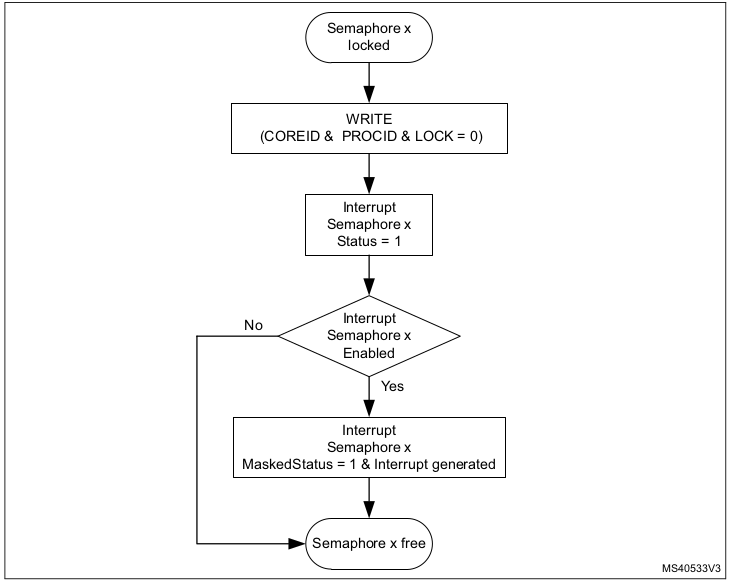
\includegraphics[width=150mm, keepaspectratio]{figures/hsem-interrupt.png}
    \caption{HSEM Interrupt State Diagram\cite{HsemInterrupt}}
    \label{fig:hsem-interrupt-sd}
\end{figure}

As an example, Listing~\ref{lst:interrupt-hsem-ex} shows the implementation of an interrupt handler that toggles an LED when any HSEM interrupt is triggered. There is only one source of interrupt for this peripheral, so one interrupt handler must serve the interrupts coming from all the semaphores. In the interrupt handler, we first query the list of masked freed semaphores then disable interrupt and finally clear the interrupt flags. After these steps, the interrupt handler can provide its normal functionality, which in this case is just toggling an LED.

\subsection{Limitations}

Dual-core functionality is not supported in underlying crates, only one of the two interrupt lines can be used. As one interrupt line is connected to each of the two cores, this means that through correct and safe code we are only able to handle HSEM interrupts on the M7 core.


\chapter{Example Application}

In this chapter, I will showcase the development of an example project that aims to demonstrate the capabilities of the selected multicore microcontroller and the Rust programming language. I will highlight features that are plain better from most perspectives, as well as the areas where this approach falls short compared to a traditional C project. The example project will have a definite function but the usage of certain peripherals and language features are more in focus thus the functionality may seem a bit purposeless as a real application.

\section{General Description}

The example application implements a very basic webserver on the M7 core of the microcontroller and does some light signal processing on the M4 core. The general direction of this project was to design one part of the application to use the ethernet peripheral in some capacity, and the other to be capable of doing a task in real time. Also I had to make sure that safe, two-way communication between the two cores is displayed in the application.

Finally, an application draft was drawn up. In it, the M7 core handles the ethernet peripheral and takes on the role of a simple web server. It hosts a simple website on a fixed IP address where coefficients of a low-pass filter can be supplied. The site also displays the average value of an ADC peripheral. The other core handles the previous ADC peripheral by performing filtering with the coefficients supplied on the website and a fixed formula. The filtered signal is emitted on a DAC peripheral with minimal latency latency. An average value is also calculated by the M4 core periodically from a configurable number of samples, this value will be displayed on the website.

\begin{figure}[!ht]
    \centering
    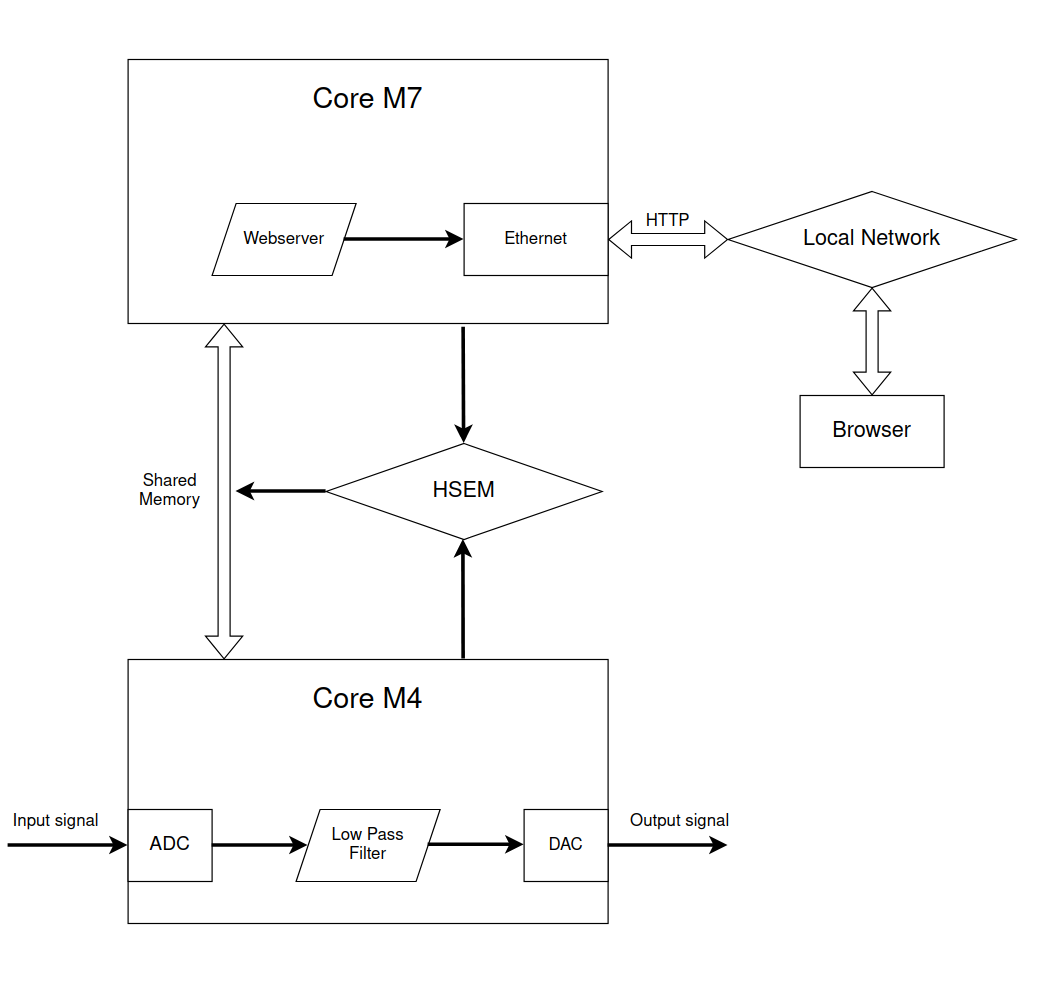
\includegraphics[width=150mm, keepaspectratio]{figures/example-app-flowchart.png}
    \caption{Block Diagram of the Example Application}
    \label{fig:app-flowchart}
\end{figure}

With this flow, the application demonstrates the usage of a decent number of peripherals, namely an ADC, a DAC, ethernet, UART, and LEDs for debugging, and of course the hardware semaphores for preventing concurrent shared memory access.

\section{Peripheral Setup}

This section demonstrates the initialization and usage of the peripherals mentioned above. Although most of these were already introduced in the previous chapter this section will focus on specific settings that facilitate this example application.

\subsection{Basic peripherals}

The basic peripherals and their usage, namely UART, LEDs, and shared memory, are already well documented in previous chapters. However, some significant changes were made to the very beginning of the program where clocks, resets, and power sources are initialized. This was necessary for two reasons. For once, different clock and reset configuration was needed if we were to use the ethernet peripheral, it needed multiple types of clock signals which are supposed to be related to each other in value. The second reason was an issue where resetting the system caused it to go into an unsteady state and behave unexpectedly, eg. only one core would work. This state could only be fixed by loading a new image onto the microcontroller.

\begin{lstlisting}[language=Rust,frame=single,float=!ht,style=customrust,label={lst:clock-config},caption={Initialization of Clocks, Resets, and Power Sources}]
    let pwr = dp.PWR.constrain();
    let pwrcfg = pwr.smps().vos0(&dp.SYSCFG).freeze();

    // link SRAM3 power state to CPU1
    dp.RCC.ahb2enr.modify(|_, w| w.sram3en().set_bit());

    // Enable HSEM clk
    dp.RCC.ahb4enr.modify(|_, w| w.hsemen().set_bit());

    let rcc = dp.RCC.constrain();
    let mut ccdr = rcc
        .sys_ck(200.MHz())
        .pll1_strategy(rcc::PllConfigStrategy::Iterative)
        .pll3_p_ck(PLL3_P)
        .hclk(200.MHz())
        .pll1_r_ck(100.MHz())
        .freeze(pwrcfg, &dp.SYSCFG);

    _cp.SCB.invalidate_icache();
    _cp.SCB.enable_icache();
    _cp.DWT.enable_cycle_counter();

    assert_eq!(ccdr.clocks.hclk().raw(), 200_000_000); // HCLK 200MHz
    assert_eq!(ccdr.clocks.pclk1().raw(), 100_000_000); // PCLK 100MHz
    assert_eq!(ccdr.clocks.pclk2().raw(), 100_000_000); // PCLK 100MHz
    assert_eq!(ccdr.clocks.pclk4().raw(), 100_000_000); // PCLK 100MHz
\end{lstlisting}

In Listing~\ref{lst:clock-config} power is enabled in the usual way, and then clock and power are enabled for the SRAM3 memory, which will be used by the ethernet driver, and the hardware semaphores. Then the clocks are configured according to ethernet examples from the \mycode{stm32h7xx-hal} crate. \cite{HalExamples} After that the instruction cache is flushed and enabled so every restart starts the MCU with a clean state in this regard. The last section asserts that all the clock signals are correctly configured for ethernet usage. Debugging issues around clocks would be a frustrating task when the code is already developed, so it is imperative that these asserts stop the execution if the clocks are incorrectly configured.

Some of the variable names are prepended with an underscore which signals to the Rust compiler that the variable is intentionally left unused. This may seem strange especially when a variable like this is used, but we have to remember that the code for the two diverges at some point and become separated at compile time. So if a variable is not used on one core, it will generate a warning even if the other core uses it. This solution is more acceptable than turning off unused variable warnings altogether.

\subsection{Ethernet}

In this section, I will demonstrate the usage of the ethernet peripheral and its driver coupled with a TCP stack.

\subsubsection{Driver}

The ethernet driver is part of the \mycode{stm32h7xx-hal} crate. this driver provides an interface for the STM32H7 microcontroller to communicate over Ethernet using the MAC and PHY components. It leverages DMA for efficient data transfer and integrates with the \mycode{smoltcp} crate, which will serve as the TCP stack, to enable networking capabilities. The driver can be used for tasks such as sending and receiving Ethernet frames, configuring MAC and PHY parameters, and interfacing with higher-level networking protocols.

The driver provides an \mycode{EthernetMAC} struct which represents the MAC (Media Access Control) layer. It initializes and configures the MAC for communication by setting up its registers. These hold various information handled by this layer such as MAC address and flow control settings. It also provides methods \mycode{smi_read()} and \mycode{smi_write()} for the SMI (Serial Management Interface) which facilitates the communication between the MAC and the external PHY registers. these methods are provided by implementing the \mycode{StationManagement} trait for the \mycode{EthernetMAC} struct.

DMA is extensively used by the ethernet driver so the CPU is not throttled by the constant flow of information that is typical to this interface. The \mycode{EthernetDMA} struct represents the Ethernet DMA engine which is responsible for managing the flow of data between memory and the MAC.
DMA descriptors, \mycode{TDes} and \mycode{RDes}, are used to control the transfer of data between the MAC and memory. The descriptors are organized in rings for efficient handling of multiple data frames. The \mycode{TDesRing} and \mycode{RDesRing} structs manage the transmit and receive descriptor rings, respectively. The \mycode{init()}, \mycode{available()}, \mycode{release()}, and \mycode{buf_as_slice_mut()} methods provide functionality for initializing, checking availability, releasing, and accessing DMA descriptors and associated buffers.

\subsubsection{Smoltcp}

The \mycode{smoltcp} crate stands as a versatile networking stack in the Rust programming language, designed to offer modularity and composability for the development of networking applications. At its core, \mycode{smoltcp} supports a range of essential networking protocols such as IPv4, IPv6, TCP, UDP, ICMP, and more. In this project, \mycode{smoltcp} is primarily used as a TCP stack in the networking schema. \cite{Smoltcp}

One of the key architectural principles of \mycode{smoltcp} lies in its abstraction of networking devices through the \mycode{phy::Device} trait. This trait serves as the interface for network devices, allowing seamless integration with different hardware or software networking implementations. This level of abstraction enhances the adaptability of \mycode{smoltcp} to various platforms and facilitates ease of use.

A notable aspect of the crate is its adherence to the Berkeley Sockets API, providing a familiar programming interface for developers well-versed in network programming. This socket API simplifies the process of building networking applications, contributing to a smoother development experience.

Still, one of the main reasons \mycode{smoltcp} is used in embedded projects like this is that it can operate using a \mycode{no_std} environment, while still providing a fairly high-level API-s.

\subsubsection{Connection to TCP stack}

The connection to the \mycode{smoltcp} crate, which serves as the TCP stack in this project, is achieved by implementing the \mycode{phy::Device} trait. The driver does this and so \mycode{smoltcp} is able to communicate with the underlying network device. Two other interfaces need implementation before our program can fully utilize the TCP stack.

First of all static storage is needed to store various data. In this project, Listing~\ref{lst:static-net-storage} fills this function. Most notably it can hold IP addresses, sockets, and routes, while also providing the TX and RX buffers for the TCP stack.

\begin{lstlisting}[language=Rust,frame=single,float=!ht,style=customrust,label={lst:static-net-storage},caption={Definition of Net Static Storage Type}]
    #[cfg(core = "0")]
    pub struct EthernetStorage<'a> {
        ip_addrs: [IpCidr; 1],
        socket_storage: [SocketStorage<'a>; 8],
        neighbor_cache_storage: [Option<(IpAddress, Neighbor)>; 8],
        routes_storage: [Option<(IpCidr, Route)>; 1],

        // network buffers
        tcp_rx_buffer_storage: [u8; MAX_PACKET_SIZE],
        tcp_tx_buffer_storage: [u8; MAX_PACKET_SIZE],
    }
\end{lstlisting}

Static storage is only the first part of the puzzle. We also need to implement the \mycode{Interface} trait from the \mycode{smoltcp} crate which consists of two functions. The \mycode{new()} function will create an instance of \mycode{Net}, which is the name for our implementation of \mycode{Interface}, by populating the previously defined static storage. The \mycode{pull()} method will poll the ethernet interface and load the RX buffers when it is triggered. It can be triggered by explicitly calling the method, or what is used in this case, a dedicated ethernet interrupt.

\begin{lstlisting}[language=Rust,frame=single,float=!ht,style=customrust,label={lst:eth-interrup-handler},caption={Ethernet Interrupt Handler}]
    #[cfg(core = "0")]
    #[interrupt]
    fn ETH() {
        unsafe { ethernet::interrupt_handler() };

        if let Some(ethernet) = unsafe { ETHERNET.as_mut() } {
            let time = ATOMIC_TIME.load(Ordering::Relaxed);
            ethernet.poll(time as i64);
        }
    }
\end{lstlisting}

\subsubsection{Usage}

Before we can start using the ethernet peripheral we first need to instantiate the types we defined before.

\begin{lstlisting}[language=Rust,frame=single,float=!ht,style=customrust,label={lst:eth-globals},caption={Global Static Variables Related to Ethernet}]
    const MAC_LOCAL: [u8; 6] = [0x02, 0x00, 0x11, 0x22, 0x33, 0x44];
    const IP_LOCAL: [u8; 4] = [192, 168, 0, 139];
    const MAX_PACKET_SIZE: usize = 576;
    const LOCAL_PORT: u16 = 6970;

    static ATOMIC_TIME: AtomicU32 = AtomicU32::new(0);
    static mut ETHERNET: Option<Net> = None;
    static mut ETHERNET_STORAGE: EthernetStorage = EthernetStorage::new();
    #[link_section = ".sram3.eth"]
    static mut ETHERNET_DESCRIPTOR_RING: ethernet::DesRing<4, 4> = ethernet::DesRing::new();
\end{lstlisting}

The first part of Listing~\ref{lst:eth-globals} contains global constants that are related to. Notice that an IP address needs to be set here because in this configuration the network stack uses a static IP address. MAC address and port can also be set here. From these settings, it can be inferred that the web server will host the website on the local address, \url{http://192.168.0.1:6970}.

The second part is more interesting. Here, the global ethernet object and the ethernet storage it uses are created. An ethernet descriptor ring is also needed to facilitate DMA transfers. With the \mycode{#[link_section = ".sram3.eth]}, it can be placed in a specific section of SRAM3 which is defined by the HAL crate.

Next, the ethernet peripheral can finally be initialized with all types and variables being defined. After the correct pins assume their appropriate modes, DNA and MAC objects are created from the static variables.

\begin{lstlisting}[language=Rust,frame=single,float=!ht,style=customrust,label={lst:eth-init},caption={Initialization of the Ethernet Peripheral}]
    let mac_addr = EthernetAddress::from_bytes(&MAC_LOCAL);
    let (eth_dma, eth_mac) = unsafe {
        ethernet::new_unchecked(
            dp.ETHERNET_MAC,
            dp.ETHERNET_MTL,
            dp.ETHERNET_DMA,
            &mut ETHERNET_DESCRIPTOR_RING,
            mac_addr.clone(),
            ccdr.peripheral.ETH1MAC,
            &ccdr.clocks,
        )
    };

    let mut lan8742a = ethernet::phy::LAN8742A::new(eth_mac.set_phy_addr(0));
    lan8742a.phy_reset();
    lan8742a.phy_init();
    while !lan8742a.poll_link() {}

    unsafe {
        ethernet::enable_interrupt();
        _cp.NVIC.set_priority(pac::Interrupt::ETH, 196); // mid prio
        cortex_m::peripheral::NVIC::unmask(pac::Interrupt::ETH);
    }

    unsafe { ETHERNET = Some(Net::new(&mut ETHERNET_STORAGE, eth_dma, mac_addr)); }
\end{lstlisting}

After that, a handler for the PHY is created and used for resetting and initializing the layer. The program then busy waits for the link to become active. At this point, the interface is ready to be used but the global ethernet object needs to be populated with relevant references, and the ethernet interrupt needs to be enabled. This is done in the last and second to last parts of Listing~\ref{lst:eth-init}.

As a final step, some references are created in the TCP stack.

\begin{lstlisting}[language=Rust,frame=single,float=!ht,style=customrust,label={lst:tcp-init},caption={Creating References for TCP Objects}]
    let store = unsafe { &mut ETHERNET_STORAGE };
    let tcp_rx_buffer = TcpSocketBuffer::new(&mut store.tcp_rx_buffer_storage[..]);
    let tcp_tx_buffer = TcpSocketBuffer::new(&mut store.tcp_tx_buffer_storage[..]);
    let tcp_socket_handle = unsafe { ETHERNET.as_mut().unwrap().interface.add_socket(TcpSocket::new(tcp_rx_buffer, tcp_tx_buffer)) };
\end{lstlisting}

\subsection{ADC}

Initializing the ADC is not as cumbersome as setting up ethernet was, it does not require any additional setup. We only need to create a handle with which the peripheral can be configured.

\begin{lstlisting}[language=Rust,frame=single,float=!ht,style=customrust,label={lst:adc-init},caption={Initialization of the ADC}]
    let mut adc1 = adc::Adc::adc1(
        dp.ADC1,
        16.MHz(),
        &mut delay,
        ccdr.peripheral.ADC12,
        &ccdr.clocks,
    ).enable();
    adc1.set_resolution(adc::Resolution::SixteenBit);
    let mut channel = gpioc.pc0.into_analog();
\end{lstlisting}

We are using the ADC1 peripheral but it is not coupled with ADC2 in this instance. The sampling time is set at 16 MHz and the resolution is sixteen bit. The channel is implicitly selected by defining which physical pin is used as analog input.

\subsection{DAC}

Configuring the DAC is an even more simple task. We only need to acquire a handler for the DAC instance, which covers both DAC modules, and calibrate the buffer. This way the default settings are used, which means that the output can be given in a 12-bit format, making the minimal value \mycode{0} and the maximal \mycode{4095}.

\begin{lstlisting}[language=Rust,frame=single,float=!ht,style=customrust,label={lst:dac-init},caption={Initialization of the DAC}]
    let dac = dp.DAC.dac(gpioa.pa4, ccdr.peripheral.DAC12);
    let mut dac = dac.calibrate_buffer(&mut delay).enable();
    dac.set_value(2048);
\end{lstlisting}

In the last line of Listing~\ref{lst:dac-init} the output value is set to the 50\% of VDDA which is configured to be 3.3 V by default.

\section{Main Loop}

In this section, I will showcase what the two cores are doing after their initialization is complete and enter their respective infinite loops.

\subsection{Webserver}

On the M7 core, a very minimalist webserver is implemented. The server will wait for a GET or POST HTTP request and send back an answer containing a simple HTML website.

\begin{lstlisting}[language=Rust,frame=single,float=!ht,style=customrust,label={lst:html-strings},caption={HTML Page Defined in a String}]
    const WEBPAGE_UPPER: &str =
    "HTTP/1.1 200 OK
    Content-Type: text/html

    <!DOCTYPE html>
    <html>
    <head>
        <title>STM32H745 Dual Core Demo App</title>
    </head>
    <body>
        <h1>STM32H745 Dual Core Demo App</h1>";

    const WEBPAGE_LOWER: &str =
    r#"
    <p>The filtering will use the formula: y[0] = alpha*u[0]+(1-alpha)*y[-1] + beta*u[-1]
    <form action="/" method="POST">
      <input type="text" id="alpha" name="alpha" placeholder="alpha">
      <input type="text" id="beta" name="beta" placeholder="beta">
      <input type="submit" value="Set">
    </form>
    </body>
    </html>"#;
\end{lstlisting}

\begin{figure}[!ht]
    \centering
    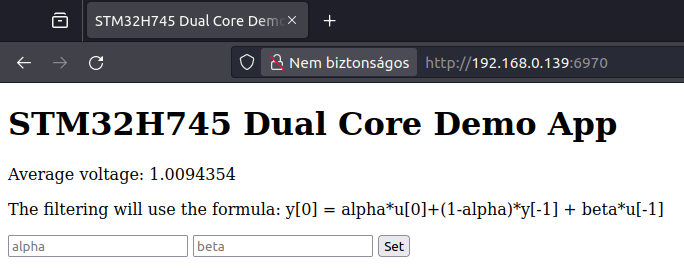
\includegraphics[width=150mm, keepaspectratio]{figures/webpage.png}
    \caption{Screenshot of the HTML Page}
    \label{fig:html-page}
\end{figure}

The HTML page is broken into an upper and lower part. The middle can contain additional elements, for example, the average value will be displayed this way. Besides that, it has a title and a form in which an alpha and a beta value can be provided. How these coefficients influence the filtering done on the other core is also displayed on the page.

As with any server using sockets, the loop of this one starts with entering a \mycode{listen()} function. Once a connection is established, the server can call a \mycode{recv()} function. The data can be received in a closure, where it can be collected into a byte array.

\begin{lstlisting}[language=Rust,frame=single,float=!ht,style=customrust,label={lst:server-recv},caption={Receiving the Contents of the TCP Buffer}]
    if !tcp_socket.is_open() {
        tcp_socket.listen(LOCAL_PORT).unwrap();
    }

    if tcp_socket.may_recv() {
        let mut headers = [httparse::EMPTY_HEADER; 16];
        let mut req = httparse::Request::new(&mut headers);
        let mut data_len = 0;
        let display_voltage;
        let data = tcp_socket.recv(|buffer| {
            let mut data = [0u8; 576];
            data_len = buffer.len();
            for i in 0..buffer.len() {
                data[i] = buffer[i];
            }
            (buffer.len(), data)
        }).unwrap();

    // ...
\end{lstlisting}

After this, the data needs to be parsed. We know that it contains an HTML request. For parsing the header part of the request, an external crate, \mycode{httparse} can be used. This crate is compatible with projects that do not use the standard library, as it does not allocate memory other than the buffer it receives the data in. \cite{Httparse} After parsing the HTTP header, all of its records are available, but here we only need the type of the request. For GET requests, the server will simply send back the HTML page to the client and close the connection. POST requests are used to update the values of the alpha and beta coefficients. The HTML page is included in the reply to the POST request too. The route of the request is not checked, so this server currently can only supply this single page, but does not require routing. All the other types of HTTP requests just cause the server to close the connection.

\begin{lstlisting}[language=Rust,frame=single,float=!ht,style=customrust,label={lst:get-post},caption={Handling of GET and POST requests}]
    let hsem_taken_by_this_core = 0x80000000u32 & ((get_core_id() as u32) << 8);
    let _res = req.parse(&data).unwrap();
    match req.method.unwrap() {
        "GET" => {
            log_serial!(tx, "In GET arm\r\n");
            hsem.r[0].read().lock().bit();
            delay.delay_ms(100u16);
            hsem.r[0].write(|w| unsafe { w
                .procid().bits(0)
                .masterid().bits(3)
                .lock().bit(false) }
            );
        }
        "POST" => {
            log_serial!(tx, "In POST arm\r\n");
            (alpha, beta) = extract_coefs(&data);
            log_serial!(tx, "Got {} and {}\r\n", alpha, beta);
            while hsem.fast_lock(0).unwrap() != hsem_taken_by_this_core {}
            unsafe {
                display_voltage = SHARED_DATA.voltage;
                SHARED_DATA.alpha = alpha;
                SHARED_DATA.beta = beta;
            }
            let _ = hsem.release(0);
        }
        _ => {
            log_serial!(tx, "In ERROR arm\r\n");
            tcp_socket.close();
        }
    }
\end{lstlisting}

The variables set in a POST request are stored in the body of the request in the format \mycode{variable1=value1&variable2=value2} and so on. These are extracted by a function that parses the body of the HTTP request. Then the hardware semaphore is taken and alpha and beta can be placed in a shared memory region, while the average voltage supplied by the other core can be extracted and prepped for display in the next step.

If the server can send it to the client it will write the HTML page into the TCP TX buffer and send it before closing the connection. The average voltage is placed between the upper and lower parts of the page with the help of the \mycode{format_args!()} macro.

\begin{lstlisting}[language=Rust,frame=single,float=!ht,style=customrust,label={lst:may-send},caption={Sending a Response to the Client}]
    if tcp_socket.may_send() {
        let webpage = write_to::show(&mut webpage,
            format_args!("{}Average voltage: {}{}", WEBPAGE_UPPER, display_voltage, WEBPAGE_LOWER))
            .unwrap()
            .as_bytes();
        tcp_socket.send_slice(webpage).unwrap();
        tcp_socket.close();
    }
\end{lstlisting}

With the connection closed, the job of this core is done and the loop can start again from the beginning with the listening phase.

\subsection{Signal Filter}

The M7 core of the microcontroller performs low pass filtering based on the coefficients supplied by a user on the webpage hosted by the other core. Samples are also saved in a buffer, and when it becomes full, an average is calculated. After this calculation, the program passes this average to the other core and takes the new values of the alpha and beta coefficients.

\begin{lstlisting}[language=Rust,frame=single,float=!ht,style=customrust,label={lst:adc-read},caption={Reading and Converting Input Voltage}]
    let reading: u32 = adc1.read(&mut channel).unwrap();
    samples[counter] = reading as f32 * (3.3 / adc1.slope() as f32);

    adc_value = samples[counter];
    filtered_value = alpha * adc_value
                     + (1.0 - alpha) * prev_filtered_value
                     + beta * prev_adc_value;

    prev_adc_value = adc_value;
    prev_filtered_value = filtered_value;
\end{lstlisting}

Listing~\ref{lst:adc-read} shows how a sample is taken from the ADC. A blocking \mycode{read()} method is called which returns the raw value extracted from the register. This is then turned into a voltage value and stored in a buffer. Then the filtering happens using the two coefficients and the formula already presented previously. Alpha values closer to zero will result in more efficient filtering, meaning the cutoff point will be closer to the lower frequencies.

\begin{lstlisting}[language=Rust,frame=single,float=!ht,style=customrust,label={lst:dac-set},caption={Setting the DAC Output Value}]
    let out_value: u16 = if filtered_value < 0.0 { 0 }
        else if filtered_value > 3.3 { 4095 }
        else { ((filtered_value /  3.3) * 4096.0) as u16};
    dac.set_value(out_value);
    for i in 0..5 {
        cortex_m::asm::nop();
    }
\end{lstlisting}

The output value is calculated by scaling the filtered value to the range of the 12-bit DAC. Also, we need to wait here for a couple of cycles according to Figure~{fig:dac-timing} to wait for the output value to settle.

Finally, when the buffer is full, an average voltage is calculated from the input voltages.

\begin{lstlisting}[language=Rust,frame=single,float=!ht,style=customrust,label={lst:avg-voltage},caption={Calculating the Average Voltage}]
    let hsem_taken_by_this_core = 0x80000000u32 & ((get_core_id() as u32) << 8);
    if counter == 1023 {
        counter = 0;
        let mut avg = 0f32;
        for v in samples { avg += v; }
        avg /= 1024.0;
        while hsem.fast_lock(0).unwrap() != hsem_taken_by_this_core {}
        unsafe {
            display_voltage = SHARED_DATA.voltage;
            SHARED_DATA.alpha = alpha;
            SHARED_DATA.beta = beta;
        }
        let _ = hsem.release(0);
    }
    counter += 1;
\end{lstlisting}

The part where shared memory is accessed is also guarded by the same hardware semaphore as it was with the other core. Note that \mycode{hsem_taken_by_this_core} is defined in exactly the same format as it was on the other core, but eventually compiles to a different value.

\chapter{Evaluation}

\section{Results}

\section{Further tasks}

%\include{content/latex-tools}
%\include{content/thesis-format}
%\include{content/template-usage}
%\include{content/task-interpretation}


% Acknowledgements
%~~~~~~~~~~~~~~~~~~~~~~~~~~~~~~~~~~~~~~~~~~~~~~~~~~~~~~~~~~~~~~~~~~~~~~~~~~~~~~~~~~~~~~
%%----------------------------------------------------------------------------
\chapter*{\koszonetnyilvanitas}\addcontentsline{toc}{chapter}{\koszonetnyilvanitas}
%----------------------------------------------------------------------------

I would like to express my deepest gratitude to my advisor, Dr. Tamás Kovácsházy, for his support and guidance during the time of this project and the my whole university journey. With his help on this project I was able to venture into a fascinating field of study that very much piqued my interest despite being relatively new.

I would also like to extend my heartfelt thanks to all my friends who supported me through ups and downs while enrolled in this master's degree program.

Finally, I extend my deepest gratitude to my mother, Zsuzsanna Katona, whose unwavering support and selfless encouragement have been a pillar of strength throughout my university journey.



% List of Figures, Tables
%~~~~~~~~~~~~~~~~~~~~~~~~~~~~~~~~~~~~~~~~~~~~~~~~~~~~~~~~~~~~~~~~~~~~~~~~~~~~~~~~~~~~~~
%\listoffigures\addcontentsline{toc}{chapter}{\listfigurename}
%\listoftables\addcontentsline{toc}{chapter}{\listtablename}


% Bibliography
%~~~~~~~~~~~~~~~~~~~~~~~~~~~~~~~~~~~~~~~~~~~~~~~~~~~~~~~~~~~~~~~~~~~~~~~~~~~~~~~~~~~~~~
\addcontentsline{toc}{chapter}{\bibname}
\bibliography{bib/mybib}


% Appendix
%~~~~~~~~~~~~~~~~~~~~~~~~~~~~~~~~~~~~~~~~~~~~~~~~~~~~~~~~~~~~~~~~~~~~~~~~~~~~~~~~~~~~~~
%----------------------------------------------------------------------------
\appendix
%----------------------------------------------------------------------------
\chapter*{\fuggelek}\addcontentsline{toc}{chapter}{\fuggelek}

The project is in a public repository available at: \newline\url{https://github.com/Goldan32/h745-start}

\setcounter{chapter}{\appendixnumber}
%\setcounter{equation}{0} % a fofejezet-szamlalo az angol ABC 6. betuje (F) lesz
\numberwithin{equation}{section}
\numberwithin{figure}{section}
\numberwithin{lstlisting}{section}
%\numberwithin{tabular}{section}


%\label{page:last}
\end{document}
